\documentclass[a4paper,12pt,oneside]{report}
\usepackage{OvidiusFMI}
\usepackage{times}
\usepackage{graphicx}
\usepackage{hyperref}
\usepackage{color,xcolor}
\usepackage{amsmath}
\usepackage{framed}
\usepackage{indentfirst}
\usepackage{enumerate}
\usepackage[shortlabels]{enumitem}
\usepackage{listings}
\usepackage{amsmath,amsfonts,amssymb,amsthm,epsfig,epstopdf,url,array}
\usepackage{multicol,multirow}
\definecolor{code}{rgb}{0.97,0.97,0.97}
\lstdefinestyle{customc}{
  belowcaptionskip=1\baselineskip,
  backgroundcolor=\color{code},
  breaklines=true,
%  frame=L,
%  xleftmargin=\parindent,
  language=C,
  showstringspaces=false,
  morekeywords={bool,
  				 glutMainLoop, glutIdleFunc, glMatrixMode, glLoadIdentity, glPushMatrix, glPopMatrix, 
  				 glBegin, glEnd, glTranslatef, glRotatef, glScalef, glColor3f, glColor4f, glutSolidCube, glutWireCube, glutSolidSphere,
  				 glutWireSphere, glutSolidCone,glutSetWindowTitle,glutGet,glClear,glutSwapBuffers,glDepthFunc,
  				 glutWireCone, glutSolidTorus, glutWireTorus, glutSolidDodecahedron, glutWireDodecahedron,
  				 glutSolidOctahedron, glutWireOctahedron, glutSolidTetrahedron, glutWireTetrahedron, 
  				 glVertex3f,glVertex2f,glPointSize,
  				 glutSolidIcosahedron, glutWireIcosahedron, glutSolidTeapot, glutWireTeapot,glutReshapeFunc,
  				 glFlush, gluPerspective, glutPostRedisplay, glutInit, glutKeyboardFunc,glutKeyboardUpFunc,
  				 glutInitWindowSize, glutInitWindowPosition, glutInitDisplayMode, glutCreateWindow, glutDisplayFunc,glutPassiveMotionFunc,
  				 glClear,glTexCoord2f,
  				 glEnable, glDisable, glLightfv, glMaterialfv, glCullFace,glViewport,
  				 glFrontFace,glColor3ub, glShadeModel,
  				 glGenLists, glGetFloatv,glGentextures,glTexImage2D,glTexParameteri, free, glDeleteTextures,
  				 glLineStipple, glLineWidth, glBindTexture,glGenTextures,
  				 glNewList, glEndList, glCallList,
  				 glMap1f,glEvalCoord1f,glMapGrid1d,glEvalMesh1,glMap2f,glEvalCoord2f,glMapGrid2f,glEvalMesh2,
  				 gluBeginTrim, gluEndTrim, gluPwlCurve,glHint,
  				 GLUnurbsObj, gluBeginSurface, gluNurbsSurface, gluEndSurface, gluNewNurbsRenderer, 									gluNurbsProperty,gluQuadricNormals,
  				 glNormal3f,
  				 gluQuadricTexture,GLUquadricObj,gluSphere,
  				 glPolygonMode, glBlendFunc,glFogi,glFogiv,glFogfv,
  				 GLfloat, GLdouble, GLint,GLuint, GLushort,GLubyte, glRasterPos2f,
  				 gluBeginCurve, gluNurbsCurve, gluEndCurve,
  				 glOrtho, gluLookAt, glutBitmapCharacter, 
  				 glInitNames, glPushName, glLoadName, glSelectBuffer, glRenderMode,gluPickMatrix, glGetIntegerv, glutMouseFunc,glutMotionFunc,system,
  				 glPushAttrib, glPopAttrib, glMultMatrixf, sprintf, glClearStencil, glStencilFunc,glStencilOp,glStencilMask,glColorMask,glActiveStencilFaceEXT,fprintf},  
%   numbers=left,                    % where to put the line-numbers; possible values are (none, left, right)
  %numbersep=5pt,                   % how far the line-numbers are from the code
  %numberstyle=\tiny\color{code}, % the style that is used for the line-numbers
  basicstyle=\footnotesize\ttfamily,
  keywordstyle=\bfseries\color{green!40!black},
  commentstyle=\itshape\color{purple!40!black},
  identifierstyle=\color{blue},
  stringstyle=\color{orange},
}

\lstset{escapechar=@,style=customc}


\newtheorem{definition}{Defini\c tie}
\newtheorem{problem}{Problema}
\newtheorem{proposition}{Propozi\c tie}
\newtheorem{demonstration}{Demonstra\c tie}
\newtheorem{example}{Exemplu}
\newtheorem{theorem}{Teorem\u a}
\newtheorem{remark}{Observa\c{t}ie}
\newtheorem{lemma}{Lem\u{a}}
\newtheorem{solve}{Rezolvare}
\newtheorem{corollary}{Corolar}
\renewcommand*{\proofname}{\rm\bf{Demonstra\c{t}ie}:}

\facultatea{Matematic\u a \c si Informatic\u a}
\specializarea{Informatic\u a}
\teza{Diserta\c{t}ie}
\titlu{Diserta\c{t}ie}
\coordonatorPrincipal{Prof. univ. Cosma Lumini\c ta}
\autor{T\u anase Ramona Elena}
\data{2021}

\begin{document}
\maketitle

\pagenumbering{roman}
\tableofcontents

\pagenumbering{arabic}
%
%
%CAPITOLUL 1
%
%
\chapter{No\c{t}iuni teoretice}

\section{Defini\c{t}ii. Propriet\u{a}\c{t}i}

Studiul funcțiilor convexe de o variabil\u {a} reala\u {a}, ofer\u{a} o imagine excelent\u {a} a frumuse\c {t}ii \c{s}i fascina\c{t}iei matematicii avansate. Vom g\u{a}si aici o mare varietate de rezultate bazate pe argumente simple \c{s}i intuitive care au aplica\c{t}ii remarcabile.

\^{I}n continuare vom nota cu I un interval nedegenerat din \(\mathbb{R}\).

\begin{definition}

O functie \(f: I \rightarrow \mathbb{R}\) se nume\c{s}te convex\u{a} dac\u{a},
\begin{displaymath}
f \left ( \left ( 1 - \lambda  \right )x + \lambda y \right )\leq \left ( 1 - \lambda  \right ) f_{\left ( x \right )} + \lambda f_{\left ( y \right )} 	\label{eq:1.1} \tag{1.1}
\end{displaymath}
pentru orice \(x\) \c{s}i \(y\) din \(I\), \c{s}i orice \(\lambda \in \left [ 0,1 \right ]\). Func\c{t}ia \(f\) se nume\c{s}te strict convex\u{a} dac\u{a} inegalitatea \ref{eq:1.1} se pastreaz\u{a}  strict\u{a} pentru orice x \c{s}i y din I, \c{s}i orice  \(\lambda \in \left ( 0,1 \right )\) . Dac\u{a} \(-f\) este convex\u{a} (respectiv stric convex\u{a}), atunci spunem c\u{a} \(f\) este concav\u{a} (respectiv strict concav\u{a}). Dac\u{a} \(f\) este \c{s}i convex\u{a} \c{s}i concav\u{a}, atunci spunem c\u{a} \(f\) este func\c{t}ie afin\u{a}.
\end{definition}

Func\c{t}iile afine sunt tocmai func\c{t}iile de forma \(mx + n\),  \(m\) \c{s}i \(n\) constante reale.
Se poate demonstra u\c{s}or faptul c\u{a} primele trei func\c{t}ii sunt convexe (dar nu sunt strict convexe) iar celelalte dou\u{a} sunt strict convexe, respectiv strict concave:
\begin{enumerate}
  \item partea pozitiv\u{a} \(x^{+} = max \left \{ x,0 \right \}\),
  \item partea negativ\u{a} \(x^{-} = max \left \{ -x,0 \right \}\),
  \item modulul \(\left | x \right | = max \left \{ -x,x \right \}\),
  \item func\c{t}ia p\u{a}tratic\u{a} \(x^{2}\)  este strict convex\u{a} pe \(\mathbb{R}\),
  \item func\c{t}ia r\u{a}d\u{a}cin\u{a} p\u{a}trat\u{a} \(\sqrt{x}\) este strict concav\u{a} pe \(\mathbb{R}_{+}\).
\end{enumerate}

Alte criterii de convexitate legate de teoria de baz\u{a} a func{t}iilor convexe vor fi prezentate \^{i}n cele ce urmeaz\u{a}.\\

Convexitatea unei funcții \(f : I\rightarrow \mathbb{R}\), înseamnă geometric faptul că, punctele de pe graficului lui  \(f|_{\left [ u,v \right ]}\) sunt sub (sau pe) coarda care unește capetele \(\left ( u , f {\left ( u \right )} \right )\)  și \(\left ( v , f {\left ( v \right )} \right )\) pentru orice \(u, v \in I, u < v\);
(vezi Fig 1.1).

Astfel inegalitatea \ref{eq:1.1} este echivalentă cu:
\begin{displaymath}
  f\left ( x \right )\leq f\left ( u \right ) +\frac{f\left ( v \right )- f\left ( u \right )}{v - u}\left ( x - u \right ) \label{eq:1.2} \tag{1.2}
\end{displaymath}
pentru orice \(x\in \left [  u, v\right ]\), și \(u, v \in I, u < v\).

\begin{center}
	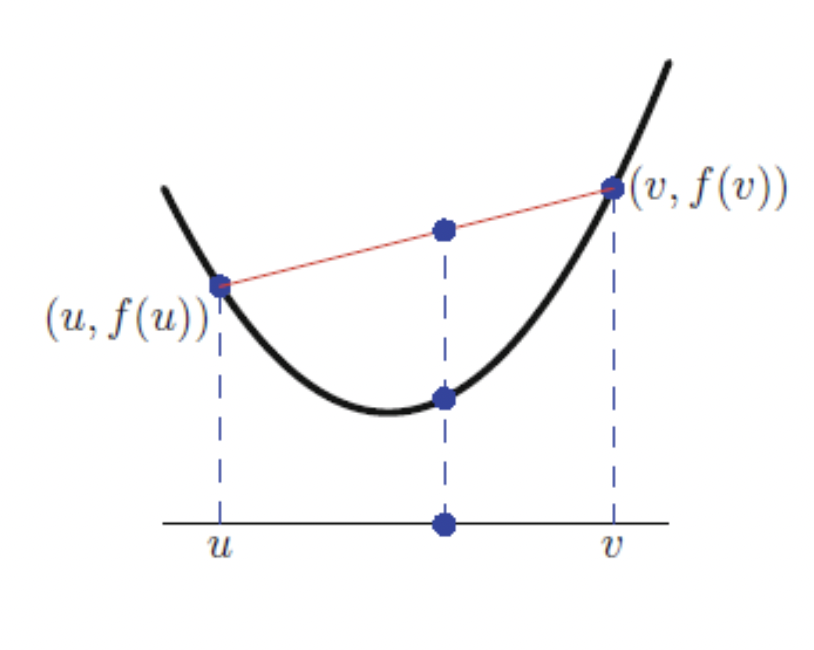
\includegraphics[width=0.5\textwidth]{fig1.1.png}
	\\ Fig 1.1 Funcții convexe: graficul este sub coarda
\end{center}

Această remarcă arată faptul ca funcțiile convexe sunt majorate de funcțiile afine pe orice subinterval compact.

Orice funcție convexa f este marginită pe fiecare subinterval compact \(\left [ u , v \right ]\) al intervalului pe care este definită. De fapt , \(f\left ( x \right ) \leq  M = max \left \{ f\left ( u \right ), f\left ( v \right ) \right \}\)  pe \(\left [ u , v \right ]\)  și scriind acest lucru într-un punct arbitrar \(x\in  \left [ u , v  \right ]\)  de forma  \(x= \frac{\left ( u + v \right )}{2} + t\) pentru  \(t\) care verifică \(\left | t \right |\leq \frac{\left ( v - u \right )}{2}\), deducem cu usurința că

\begin{displaymath}
  f\left ( x \right )=  f\left ( \frac{u+v}{2} + t\right )\geq 2 f\left ( \frac{u + v}{2} \right )- f\left ( \frac{u + v}{2} - t\right )\geq 2f\left ( \frac{u+v}{2} \right ) - M.
\end{displaymath}

\begin{theorem}
O funcție convexă \(f: I \rightarrow \mathbb{R}\) este continuă în orice punct interior al lui \(I\). 	
\end{theorem}
\begin{proof}
	Presupunem că \(a\in I\) și alegem \(\varepsilon > 0\) astfel încat \(\left [ a - \varepsilon , a + \varepsilon  \right ] \subset I\).
 Atunci
\begin{displaymath}
  f\left ( a \right )\leq \frac{1}{2} f\left ( a - \varepsilon  \right ) + \frac{1}{2}f \left ( a + \varepsilon  \right )
\end{displaymath}
și
\begin{displaymath}
  f\left ( a \pm t\varepsilon  \right )= f\left ( \left ( 1 - t \right ) a + t\left ( a \pm \varepsilon  \right )\right )\leq \left ( 1 - t \right )f\left ( a \right ) + tf\left ( a\pm \varepsilon  \right )
\end{displaymath}
pentru orice \(t\in \left [ 0 , 1 \right ]\). Prin urmare
\begin{displaymath}
  t\left ( f\left ( a\pm \varepsilon  \right ) - f\left ( a \right ) \right )\geq f\left ( a\pm t\varepsilon  \right )- f\left ( a \right )\geq -t\left ( f\left ( a\mp \varepsilon  \right ) - f\left ( a \right )\right )
\end{displaymath}
care ne conduce la
\begin{displaymath}
\left | f\left ( a\pm t\varepsilon  \right )- f\left ( a \right ) \right |\leq t max \left \{ \left | f\left ( a-\varepsilon  \right )- f\left ( a \right ) \right |, \left | f\left ( a+\varepsilon  \right ) - f\left ( a \right )\right | \right \},
\end{displaymath}
 pentru orice \(t\in \left [ 0 , 1 \right ]\). Continuitatea funcției \(f\) este acum clară.
 \end{proof}

 \begin{remark}
	Exemple simple precum, \(f\left ( x \right )= 0\) dacă \(x\in \left ( 0 , 1 \right )\), și  \(f\left ( 0 \right )= f\left ( 1 \right ) = 1\), arată faptul că salturi  pot apărea în capetele intervalului de definiție al unei funcții convexe. Totuși, aceste posibile discontinuități pot fi înlăturate.
\end{remark}


\begin{proposition}
Dacă \(f: \left [ a, b \right ]\rightarrow \mathbb{R}\) este o funcție convexă, atunci limitele
\[
f\left ( a+ \right ) = \lim_{x\rightarrow a, x> a}f\left ( x \right ),~~ f\left ( b- \right ) = \lim_{x\rightarrow b, x< b}f\left ( x \right )\] există în \(\mathbb{R}\) și
\begin{displaymath}
  \tilde{f}\left ( x \right )= \left\{\begin{matrix}
f\left ( a+ \right ) & \\
 f\left ( x \right )& \\
 f\left ( b- \right )&
\end{matrix} \begin{matrix}
\text{dacă } x=a & \\
\text{dacă } x\in \left ( a,b \right ) & \\
\text{dacă } x= b&
\end{matrix}\right.
\end{displaymath}
 este o funcție convexă continuă.
\end{proposition}
	Acest rezultat este o consecință a următoarelor rezultate :
\begin{lemma}

Dacă \(f: I \rightarrow \mathbb{R}\) este convexă, atunci sau \(f\) este monotonă pe intervalul \(I\), sau există un punct \(\xi \in int I\) astfel încat \(f\) este descrescătoare pe intervalul \(\left ( -\infty , \xi  \right )\cap I\) și crescătoare pe intervalul \(\left[\xi , \infty  \right )\cap I\).
\end{lemma}
\begin{proof}
Luăm \(a < b\) puncte interioare arbitrare ale lui \(I\) și fie
\[m = inf\left \{ f\left ( x \right ): ~~x\in \left [ a,b \right ]\right \}.\] Cum \(f\) este continuă pe \(\left [ a,b \right ]\), acest infimum este atins în punctul \(\xi \in \left [ a,b \right ]\), adică
$
  m = f\left ( \xi  \right )
$
Dacă \(a \leq x <  y< \xi\), atunci \(y\) este o combinație convexă a lui \(x\) și \(\xi\), mai exact, \[y = \frac{\xi -y}{\xi -x}x + \frac{y - x}{\xi -x}\xi.\] Cum \(f\) este convexă,
\begin{displaymath}
  f\left ( y \right )\leq \frac{\xi -y}{\xi -x}f\left ( x \right )+ \frac{y-x}{\xi -x}f\left ( \xi  \right )\leq f\left ( x \right ).
\end{displaymath}
Demonstrația se incheie cu un proces de lipire (la stanga lui \(a\) și la dreapta lui \(b\)), observând că proprietatea de covexitate face imposibilă existența a trei numere \(u < v < w\) in \(I\) astfel încat \(f\left ( u \right ) < f\left ( v \right )> f\left ( w \right )\).
\end{proof}

\begin{corollary}
\begin{enumerate}[a)]
\item Orice funcție convexț \(f: I \rightarrow \mathbb{R}\) care nu este monotonă pe
intervalul \(I\) are un minim global interior.
\item Dacă o funcție convexă \(f: \mathbb{R} \rightarrow \mathbb{R}\) este marginită superior, atunci este constantă.
\end{enumerate}
\end{corollary}
Atingere supremului la capete nu este o proprietate caracteristică a funcțiilor convexe, dar avem însă urmatorul rezultat.

\begin{theorem}

Fie \(f: I \rightarrow \mathbb{R}\). Atunci \(f\) este (strict) convexă daca și numai dacă pentru orice subinterval compact \(J\) al lui \(I\), și fiecare funcție afină \(L\), supremul lui \(f+L\) pe \(J\) este atins într-un capăt al intervalului (și doar acolo).
\end{theorem}

\begin{proof}
Ne vom restrange la cazul funcțiilor convexe. Cazul funcțiilor strict convexe poate fi tratat în acelasi mod.

\textbf{Necesitatea:} Dacă \(f\) este convexă, la fel este și suma \(F = f + L\). Cum orice punct al unui subinterval \(J = \left [ x , y \right ]\) este o combinație convexă \(z = \left ( 1 - \lambda  \right )x + \lambda y \) a lui \(x\) și \(y\), avem
\begin{equation*}
\begin{split}
  \sup_{z\in J}F\left ( z \right ) &= \sup_{\lambda \in \left [ 0 , 1 \right ]}F\left ( \left ( 1 - \lambda  \right )x + \lambda y \right )\\
  &\leq \sup_{\lambda \in \left [ 0,1 \right ]}\left [ \left ( 1-\lambda  \right )F\left ( x \right ) + \lambda F\left ( y \right ) \right ] + max \left \{ F\left ( x \right ), F\left ( y \right ) \right \}
  \end{split}
\end{equation*}

\textbf{Suficiența:} Având un subinterval \(J = \left [ x,y \right ]\) al lui \(I\), există o funcție afină \(L\left ( x \right ) = mx + n\) care este egală cu \(f\) în cele doua puncte  \(x\) si \(y\).
Atunci
\begin{displaymath}
  \sup_{\lambda \in \left [ 0,1 \right ]}\left [ \left ( f - L \right )\left ( 1 - \lambda  \right )x + \lambda y \right ] = 0,
\end{displaymath}
care ne conduce la
\begin{displaymath}
  0\geq f\left ( \left ( 1 - \lambda  \right )x + \lambda y \right )- L\left ( \left ( 1 - \lambda  \right )x - \lambda L \right )
\end{displaymath}
  \begin{displaymath}
  = f\left ( \left ( 1 - \lambda  \right )x + \lambda y  \right ) - \left ( 1 - \lambda  \right )L\left ( x \right ) - \lambda L\left ( y \right )
\end{displaymath}
\begin{displaymath}
  = f\left ( \left ( 1 - \lambda  \right )x + \lambda y \right ) - \left ( 1 - \lambda  \right ) f\left ( x \right ) - \lambda f \left ( y \right ),
\end{displaymath}
pentru orice \(\lambda \in \left [ 0,1 \right ]\).
\end{proof}

\begin{definition}
O funcție \(f: I \rightarrow \mathbb{R}\) se numește cvasiconvexă dacă,
 \begin{displaymath}
  f\left ( \left ( 1-\lambda  \right )x + \lambda y \right )\geq  min\left \{ f\left ( x \right ), f\left ( y \right ) \right \}
\end{displaymath}
pentru orice  \(x, y \in I\) și \(\lambda  \in \left ( 0,1 \right ]\).
\end{definition}
	 Avem următoarea caracterizare a convexității în cadrul clasei funcțiilor continue care se dovedește utilă și în verificarea convexității.
\begin{theorem}
O funcție \(f : I \rightarrow \mathbb{R}\) este convexă dacă și numai dacă ea verifică urmatoarele două condiții:
\begin{enumerate}[a)]
\item \(f\) este continuă în fiecare punct din interiorul lui \(I\); și
\item \(f\) este convexă în punctul de mijloc , adică,
\end{enumerate}
\begin{displaymath}
  f\left ( \frac{x+y}{2} \right )\leq \frac{f\left ( x \right )+f\left ( y \right )}{2}, \text{ pentru orice } x, y \in I.
\end{displaymath}
\end{theorem}
\begin{proof}
\textbf{Necesitatea }rezultă din teorema 1.1.2.

\textbf{Suficiența} o vom demonstra prin reducere la absurd. Dacă \(f\) nu este convexă, atunci există un interval \(\left [ a,b \right ]\) astfel încat graficul funcției \(f\) restricționată la  \(\left [ a,b \right ]\) să nu fie sub coarda care unește punctele \(\left ( a, f\left ( a \right ) \right )\) și \(\left ( b, f\left ( b \right ) \right )\); ca urmare , funcția
\begin{displaymath}
  \varphi \left ( x \right )= -f\left ( x \right ) + f\left ( a \right )+ \frac{f\left ( b \right )- f\left ( a \right )}{b-a}\left ( x-a \right ), x\in \left [ a,b \right ]
\end{displaymath}
are  \(\gamma = inf \left \{ \varphi \left ( x \right ) : x\in \left [ a,b \right ]\right \}< 0\).

Observam că \(-\varphi\) este convexă în punctul de mijloc, continuă și \(\varphi \left ( a \right ) =\varphi \left ( b \right ) = 0\). Fie \(c = inf \left \{ x \in \left [ a,b  \right ] : \varphi \left ( x \right )= \gamma \right \} \), atunci \(\varphi \left ( c \right ) = \gamma\)  și \(c \in \left ( a,b  \right )\). Conform definiției lui \(c\), pentru orice \(h>0\) pentru care \(c\pm h\in \left ( a,b \right )\) avem
\begin{displaymath}
  \varphi \left ( c - h  \right )> \varphi \left ( c \right ) si \varphi \left ( c + h  \right )\geq  \varphi \left ( c \right )
\end{displaymath}

Astfel
\begin{displaymath}
  -\varphi \left ( c \right )> \frac{-\varphi \left ( c-h \right )-\varphi \left ( c+h \right )}{2},
\end{displaymath}
ceea ce este în contradicție cu faptul că \(-\varphi\) este convexă în punctul de mijloc.
\end{proof}


\begin{corollary}
Fie \(f: I \rightarrow \mathbb{R}\) o funcție continuă. Atunci, \(f\) este convexă daca și numai dacă
\begin{displaymath}
  f\left ( x+h \right )+ f\left ( x - h \right ) - 2f\left ( x \right )\geq 0
\end{displaymath}
pentru orice \(x \in I\) și orice \(h > 0\) astfel încat și \(x + h\) și \(x - h\) aparțin lui \(I\).
\end{corollary}
\begin{remark}
Observăm că și Teorema 1.1.8 și Corolarul acesteia 1.1.9 de mai sus, admit variante în cazul funcțiilor strict convexe,
Corolarul 1.1.9 ne permite să verificăm imedat convexitatea / concavitatea strictă a unor funcții elementare, precum funcția exponențială, cea logaritmică, și restricția funcției sinus pe \(\left [ 0 , \pi \right ]\).

Într-adevar, pentru funcția exponențială, faptul că  \(a , b > 0, a\neq b\), implica \(\frac{a + b}{2}> \sqrt{ab}\)
este echivalentă cu
\(e^{x + h} + e^{x - h } - 2e^{x}> 0\)
pentru orice \(x\in \mathbb{R}\) și orice \(h > 0\).
\end{remark}
	Multe alte exemple pot fi deduse folosind următoarele proprietăți ale funcțiilor convexe / concave.

\begin{proposition}
\textbf{Operații cu funcții convexe:}
\begin{enumerate}[a)]
\item Adunând două funcții convexe ( definite pe același interval) obținem o funcție convexă; dacă una dintre ele este strict convexă, atunci suma lor este de asemenea strict convexă.
\item Înmulțind o funcție (strict) convexă cu un scalar (strict)  pozitiv obținem de asemenea o funcție (strict) convexă.
\item Presupunem că f și g sunt două funcții convexe pozitive definite pe un interval I. Atunci, produsul lor este o funcție convexă pe I dacă sunt sincrone în sensul că, \begin{displaymath}
   \left ( f\left ( x \right ) - f\left ( y \right ) \right )\left ( g\left ( x \right ) - g\left ( y \right )\right )\geq 0
\end{displaymath} pentru orice \(x , y \in \mathbb{R}\); de exemplu , această condiție apare daca f și g sunt amandouă descrescătoare sau amândouă crescătoare.
\item Restricția unei funcții (strict) convexe pe I, la un subinterval al lui I este de asemenea o funcție (strict) convexă.
\item Presupunem că \(f\) este o funcție bijectivă între două intervale \(I\) si \(J\). Dacă \(f\) este strict crescătoare, atunci \(f\) este (strict) convexă dacă și numai dacă \(f^{-1}\) este (strict) concavă. Dacă \(f\) este o funcție bijectivă descrescătoare, atunci \(f\) și  \(f^{-1}\) sunt ambele convexe sau ambele concave.
\item Dacă \(f\) este o funcție strict pozitivă concavă, atunci \(\frac{1}{f}\) este o funcție convexă. Aici rolul concavității și al convexității nu poate fi schimbat unul cu celălalt.
\item Maximul a doua funcții (stricte) convexe \(f , g : I \rightarrow \mathbb{R}\),
\begin{displaymath}
  max \left \{ f , g \right \}\left ( x \right )=  max \left \{ f\left ( x \right ), g\left ( x \right ) \right \}
\end{displaymath} este de asemenea o funcție (strict) convexă.
\item Compunerea \(f\left ( ax + b \right )\), a unei funcții \(f\) convexe și a unei funcții afine \(ax+b\), este o funcție convexă.
\end{enumerate}
\end{proposition}
În continuare, vom discuta extinderea inegalității convexității (1.1). În primul rand, observăm faptul că intervalele sunt închise la combinații convexe arbitrare, adică,
\begin{displaymath}
  \sum_{ k= 1}^{n}\lambda _{k}x_{k} \in I~~\mbox{pentru orice}~~x_{1},\cdots, x_{n} \in I  ~~\mbox{și orice}~~\lambda _{1},\cdots, \lambda _{n} \in \left [ 0 , 1  \right ]
\end{displaymath}
 cu \(\sum_{k = 1}^{n} \lambda _{k} = 1\).

 Acest lucru poate fi demonstrat prin inducție după \(n\).

 Cazul \(n=1\) este trivial, în timp ce \(n = 2\) rezultă din definiția unei mulțimi convexe.

  Presupunând faptul că rezultatul este adevărat pentru toate combinațiile convexe cu cel mult \(n\geq 2\) puncte, să trecem la cazul combinațiilor cu \(n + 1\) puncte, \(x = \sum_{k = 1}^{n + 1} \lambda _{k}x_{k}\). Cazul non-trivial este atunci cand toți coeficienții \(\lambda _{k}\) se află în \(\left ( 0 , 1 \right )\). Dar în acest caz, datorită ipotezei de inducție, x poate fi reprezentat ca o combinație convexă de doua elemente ale lui \(I\),
\begin{displaymath}
  x = \left ( 1 - \lambda _{n + 1} \right )\left ( \sum_{k = 1}^{n} \frac{\lambda _{k}}{1 - \lambda _{n + 1}} x_{k}\right ) + \lambda _{n + 1}x_{n + 1},
\end{displaymath}
prin urmare x apartine lui \(I\).
	Observația de mai sus asupra intervalelor are o echivalență remarcabilă pentru funcțiile convexe:

\begin{lemma}
\textbf{Cazul discret al inegalității lui Jensen}

O funcție cu valori reale \(f\) definită pe un interval \(I\) este convexă dacă și numai dacă pentru orice puncte \(x_{1},\cdots,x_{n}\) din \(I\) și orice scalari \(\lambda _{1},\cdots,\lambda _{n}\) din \(\left [ 0 , 1 \right ]\) cu \(\sum_{k = 1}^{n}\lambda _{k}= 1\) avem,
\begin{displaymath}
  f\left ( \sum_{k = 1}^{n} \lambda _{k}x_{k}\right )\leq \sum_{k = 1}^{n}\lambda _{k}f\left ( x_{k} \right ).
\end{displaymath}

Dacă \(f\) este strict convexă, inegalitatea de mai sus este strictă dacă punctele \(x_{k}\) nu sunt toate egale între ele , și scalarii \(\lambda _{k}\) sunt toți pozitivi.
\end{lemma}
\begin{proof}
Prima afirmație rezultă prin inducție matematică.

În ceea ce privește cea de a doua afirmație, presupunem că funcția \(f\) este strict convexă și
\begin{displaymath}
  f\left ( \sum_{k = 1}^{n} \lambda _{k}x_{k}\right )=  \sum_{k = 1}^{n}\lambda _{k}f\left ( x_{k} \right ). \label{eq:1.3} \tag{1.3}
\end{displaymath}
pentru  punctele \(x_{1}, \cdots, x_{n} \in I\) și scalarii \(\lambda _{1}, \cdots, \lambda _{n} \in \left ( 0 , 1\right )\) care au suma egala cu \(1\). Dacă \(x_{1}, \cdots, x_{n}\) nu sunt toți egali, mulțimea
\[S = \left \{ k: x_{k}<  max \left \{ x_{1,\cdots,x_{n}} \right \} \right \}\]
 va fi o submulțime proprie a mulțimii  \(\left \{ 1,\cdots,n \right \}\) și \(\lambda _{S} = \sum_{k \in S}^{}\lambda _{S} \in \left ( 0,1 \right )\). Cum \(f\) este strict convexă avem,
\begin{displaymath}
  f\left ( \sum_{k=1}^{n}\lambda _{k}x_{k} \right ) = f\left ( \lambda _{S}\left ( \sum_{k\in S}^{}\frac{\lambda _{k}}{\lambda _{S}} x_{k}\right ) +\left ( 1-\lambda _{S} \right )\left ( \sum_{k\notin S}^{} \frac{\lambda _{k}}{1 - \lambda _{S}}x_{k}\right )\right ) <
\end{displaymath}
\begin{displaymath}
  \lambda _{S}f\left ( \sum_{k\in S}^{}\frac{\lambda _{k}}{\lambda _{S}} x_{k}\right ) +\left ( 1 - \lambda _{S} \right )f\left ( \sum_{k\notin S}^{}\frac{\lambda _{k}}{1 - \lambda _{S}} x_{k}\right ) <
\end{displaymath}

\begin{displaymath}
  \lambda _{S} \sum_{k\in S}^{}\frac{\lambda _{k}}{\lambda _{S}} f\left ( x_{k} \right ) +\left ( 1 - \lambda _{S} \right ) \sum_{k\notin S}^{}\frac{\lambda _{k}}{1 - \lambda _{S}}f\left ( x_{k} \right )= \sum_{k=1}^{n}\lambda _{k}f\left ( x_{k} \right ),
\end{displaymath}
care contrazice ipoteza noastră \ref{eq:1.3}. Astfel, toate punctele \(x_{k}\) ar trebui să coincidă.
\end{proof}

O consecință imediată a lemei 1.1.11 (când este aplicată funcției exponențiale) este urmatorul rezultat care extinde bine cunoscuta inegalitate MA-MG (adica inegalitatea dintre media aritmetică și cea geometrică).


\begin{theorem}
\textbf{Forma ponderată a inegaliățtii mediilor}

Dacă \(x_{1},\cdots,x_{n}\in \left ( 0,\infty  \right ) si \lambda_{1},\cdots,\lambda _{n} \in \left ( 0 , 1 \right ), \sum_{k = 1}^{n}\lambda _{k}= 1\), atunci
\begin{displaymath}
  \sum_{k = 1}^{n}\lambda _{k}x_{k}> x_{1}^{\lambda _{1}}\cdots x_{n}^{\lambda _{n}}
\end{displaymath}
în afară de cazul când \(x_{1} = \cdots = x_{n}\).
	
	Înlocuind \(x_{k}\) cu \(\frac{1}{x_{k} }\) în ultima inegalitate, obținem
\begin{displaymath}
  x_{1}^{\lambda _{1}}\cdots x_{n}^{\lambda _{n}}> \frac{1}{\sum_{k = 1}^{n}\lambda _{k}\frac{1}{x_{k}}}
\end{displaymath}
în afară de cazul când \(x_{1} = \cdots = x_{n}\).
\end{theorem}
Aceasta reprezintă forma ponderată a inegalității mediei geometrice – mediei armonice (adica inegalitatea MG-MH).

Pentru \(\lambda _{1} = \cdots =\lambda _{n}= \frac{1}{n}\) obținem inegalitatea obișnuită care afirmă că pentru orice \(x_{1},\cdots,x_{n}\)  numere pozitive, nu toate egale, avem

\begin{displaymath}
  \frac{x_{1}+\cdots+x_{n}}{n}> \sqrt[n]{x_{1}\cdots x_{n}}> \frac{n}{\left ( \frac{1}{x_{1}}+\cdots+\frac{1}{x_{n}} \right )}.
\end{displaymath}




\section{Inegalitatea lui Young și consecințele sale}

Următoarul caz special al formei ponderate a inegalității MA-MG este cunoscută sub numele de inegalitatea lui Young:
\begin{displaymath}
  ab \leq \frac{a^{p}}{p}+ \frac{b^{q}}{q},
\end{displaymath}
pentru orice \(a,b \geq 0\)
și pentru orice  \(p,q \in \left ( 0 , 1 \right )\) cu proprietatea că \(\frac{1}{p}+\frac{1}{q} = 1\).
Egalitatea are loc dacă și numai dacă \(a^{p}= b^{q}\).

Inegalitatea lui Young poate fi de asemenea obținută ca o consecină a convexității stricte a funcției exponențiale.

Într-adevar
\begin{displaymath}
  ab = e^{\log_{a}b}= e^{\left (\frac{1}{p}  \right )\log_{a}p+ \left ( \frac{1}{q} \right )\log_{b}q}
< \frac{1}{p}e^{\log_{a}p}+\frac{1}{q}e^{\log_{b}q}= \frac{a^{p}}{p}+\frac{b^{q}}{q},
\end{displaymath}
pentru orice \(a,b>0\) astfel incat \(a^{p}\neq b^{q}\).

O altă soluție este oferită de studiul variației funcției diferențiabile
\begin{displaymath}
  F\left ( a \right )= \frac{a^{p}}{p}+\frac{b^{q}}{q} - ab,~ a\geq 0,
\end{displaymath}
unde \(b\geq 0\) este un paramentru. Această funcție iși atinge punctul de minim global strict în \(a= b^{\frac{q}{p}}\), care ne conduce la \(F\left ( a \right )> F\left ( b^{\frac{q}{p}} \right ) = 0\) pentru orice \(a\geq 0, a\neq b^{\frac{q}{p}}\).

	W.H.Young a dovedid de fapt  o inegalitate mult mai generală, pentru \(f\left ( x \right )=  x^{p-1}\).

\begin{theorem}
\textbf{Inegalitatea lui Young
}
Presupunem că \(f: \left [ 0,\infty  \right ) \rightarrow \left [ 0,\infty  \right )\) este o funcție continuă strict crescătoare astfel încat \(f\left ( 0 \right )= 0\) si \(\lim_{x\rightarrow \infty }f\left ( x \right )= \infty\). Atunci
\begin{displaymath}
  uv\leq \int_{0}^{u}f\left ( x \right )dx + \int_{0}^{v}f^{-1}\left ( y \right )dy
\end{displaymath}
pentru orice \(u,v\geq 0\) cu egalitate dacă și numai dacă \( v = f\left ( u \right )\).
\end{theorem}
\begin{center}
	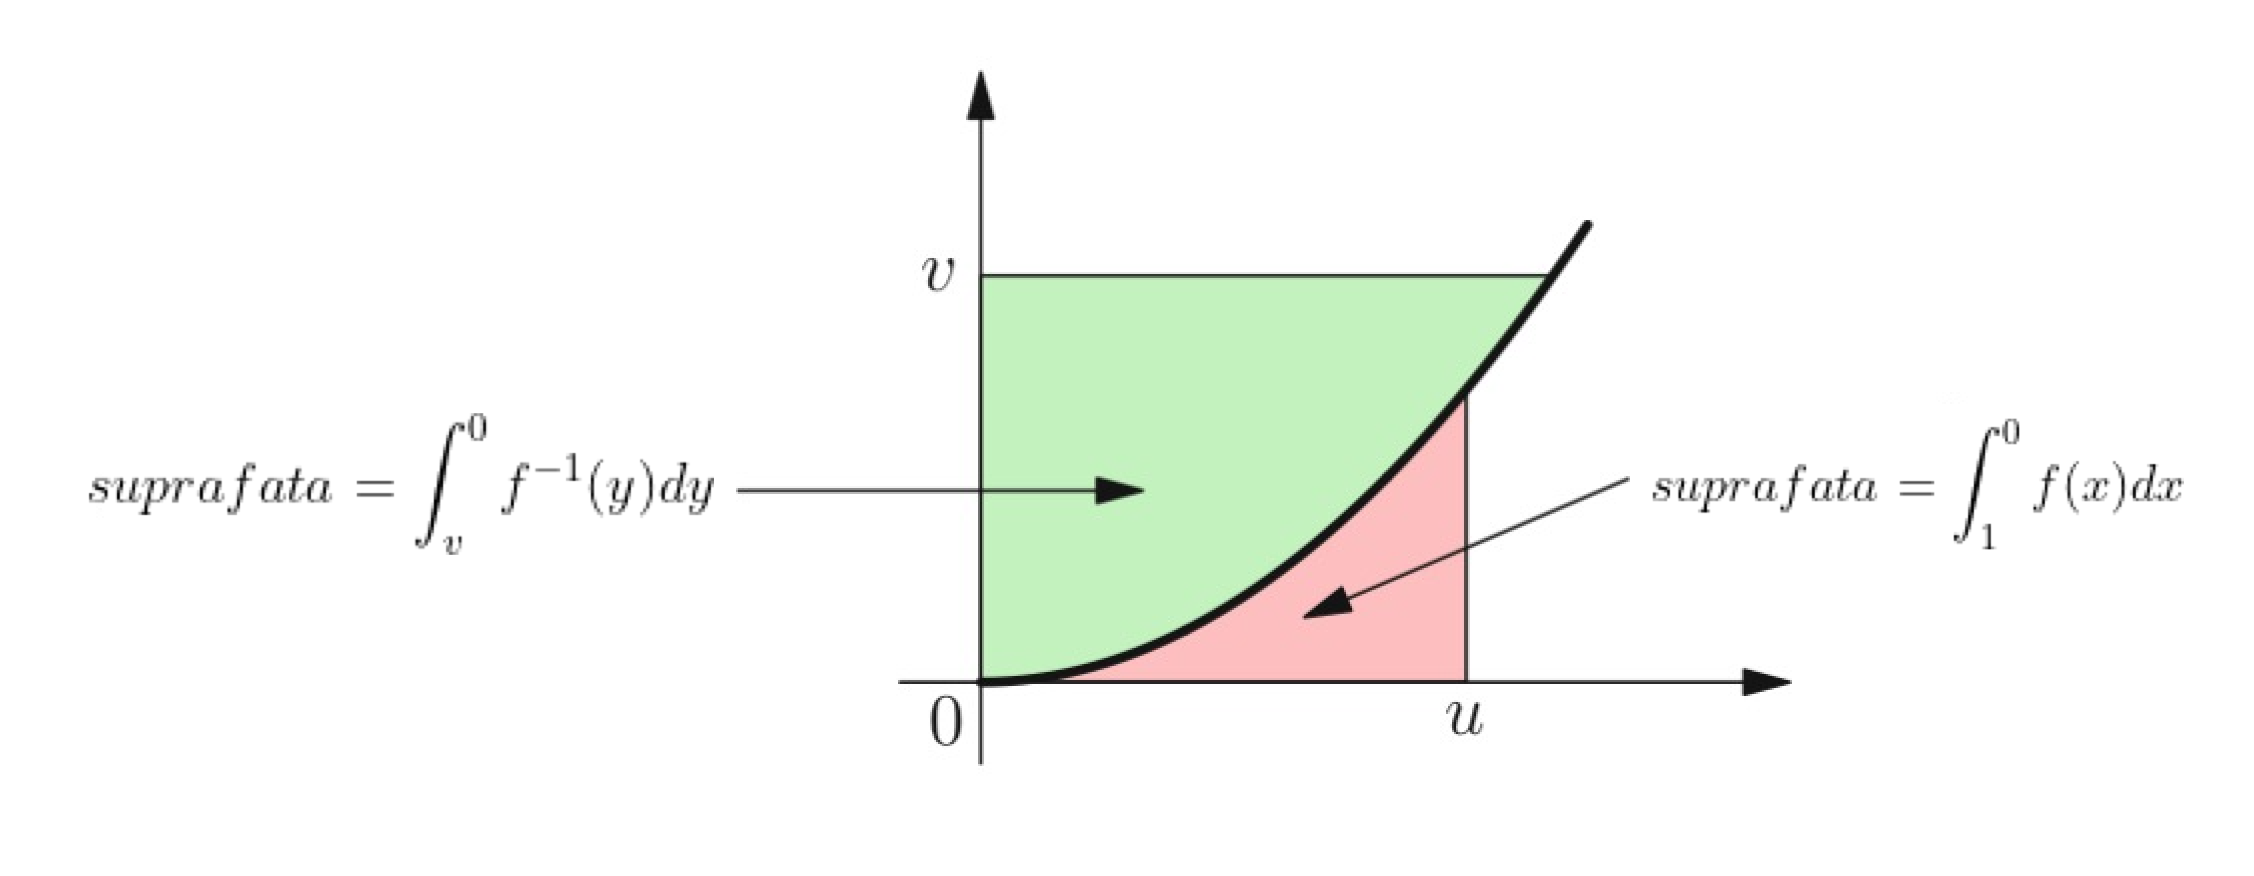
\includegraphics[width=1.0\textwidth]{fig1.2.png}
	\\ Fig 1.2 Aria  de unire a celor doua triunghiuri curbilinii depășește aria dreptunghiului cu laturile u si v
\end{center}

\begin{proof}
Folosind definitia derivatei se poate demonstra cu usurinta ca functia
\begin{displaymath}
  F\left ( u \right )= \int_{0}^{u}f\left ( x \right )dx + \int_{0}^{f\left ( u \right )}f^{-1}\left ( y \right )dy -uf\left ( u \right ), u \in \left [ 0,\infty  \right )
\end{displaymath}
este diferentiabila, cu \({F}'\) $\equiv 0.$ Astfel, \(F\left ( u \right )= F\left ( 0 \right )= 0\) pentru orice \(u\geq 0\).
	
Daca \(u, v \geq 0\)  si \(v\geq f\left ( u \right )\), atunci
\begin{displaymath}
  uv = uf\left ( u \right )+ u\left ( v- f\left ( u \right ) \right )=  \int_{0}^{u}f\left ( x \right )dx + \int_{0}^{f\left ( u \right )}f^{-1}\left ( y \right )dy + u\left ( v - f\left ( u \right ) \right ) =
\end{displaymath}

\begin{displaymath}
  = \int_{0}^{u}f\left ( x \right )dx + \int_{0}^{v}f^{-1}\left ( y \right )dy + \left [ u\left ( v-f\left ( u \right )  \right ) - \int_{f\left ( u \right )}^{v}f^{-1}\left ( y \right )dy\right ]\leq
\end{displaymath}

\begin{displaymath}
  \leq \int_{0}^{u}f\left ( x \right )dx + \int_{0}^{v}f^{-1}\left ( y \right )dy.
\end{displaymath}



	Cealalt caz, unde \(v\leq f\left ( u \right )\) poate fi tratat similar.
\end{proof}

\begin{theorem}

\textbf{Inegalitatea lui Rogers-Hölder pentru} \(p > 1\)

Fie \(p,q \in \left ( 1, \infty  \right )\) cu \(\frac{1}{p} + \frac{1}{q} = 1\) si  \(f\in L^{p}\left ( \mu  \right )\) si \(g\in L^{q}\left ( \mu  \right )\). Atunci \(fg\) apartine lui \(L^{1}\left ( \mu  \right )\) si avem
\begin{displaymath}
  \left | \int_{\Omega}^{} fg  d\mu \right |\leq \int_{\Omega}^{}\left | fg \right |d\mu \label{eq:1.6} \tag{1.6}
\end{displaymath}
si
\begin{displaymath}
  \int_{\Omega}^{}\left | fg \right |d\mu \leq \left \| f \right \|_{L^{p}}\left \| g \right \|_{{L}^{q}}. \label{eq:1.7} \tag{1.7}
\end{displaymath}
Ca o consecinta
\begin{displaymath}
  \left | \int_{\Omega}^{} fg  d\mu \right |\leq \left \| f \right \|_{L^{p}}\left \| g \right \|_{{L}^{q}}. \label{eq:1.8} \tag{1.8}
\end{displaymath}
\end{theorem}

\begin{remark}
	Rezultatul de mai sus se extinde intr-o maniera directa la perechi de forma \(p = 1, q = \infty\) si \(p = \infty, q = 1\).
	
Din Inegalitatea Rogers – Hölder rezulta ca pentru orice \(p, q, r \in \left ( 1 , \infty  \right )\) cu \(\frac{1}{p} + \frac{1}{q} = 1\) si orice \(f\in L^{p}\left ( \mu  \right )\) si \(g\in L^{q}\left ( \mu  \right )\) avem \(fg\in L^{r}\left ( \mu  \right )\) si
\begin{displaymath}
  \left \| fg \right \|_{L^{r}}\leq \left \| f \right \|_{L^{p}}\left \| g \right \|_{L^{q}} \label{eq:1.9} \tag{1.9}
\end{displaymath}


Inegalitate \ref{eq:1.8}, pentru \(p = q = 2\), este cunoscut ca \textbf{inegalitatea Cauchy-Bunyakovsky-Schwarz} pentru integrale.
\end{remark}
\begin{proof}
Prima inegalitate este triviala.

Daca \(f\) sau \(g\) sunt \(0~~ \mu\) – aproape peste tot, atunci cea de a doua inegalitate este triviala. Altfel, folosind inegalitatea lui Young, avem
\begin{displaymath}
  \frac{\left | f\left ( x \right ) \right |}{\left \| f \right \|_{L^{p}}} \cdot \frac{\left | g\left ( x \right ) \right |}{\left \| g \right \|_{L^{q}}}\leq \frac{1}{p}\cdot \frac{\left | f\left ( x \right ) \right |^{p}}{\left \| f \right \|^{p}_{L^{p}}} + \frac{1}{q}\cdot \frac{\left | g\left ( x \right ) \right |^{q}}{\left \| g \right \|^{q}_{L^{q}}}
\end{displaymath}
 pentru orice \(x\) din \(\Omega\). Astfel deducem ca \(fg \in L^{1}\left ( \mu  \right )\). De asemenea
\begin{displaymath}
  \frac{1}{\left \| f \right \|_{L^{p}}\left \| g \right \|_{L^{q}}}\int_{\Omega }\left | fg \right |d\mu \leq 1.
\end{displaymath}
\end{proof}

\begin{remark}

Conditii pentru egalitatea din Teorma 1.2.2

Observatia de baza este faptul ca  \(f\geq 0\) si \(\int_{\Omega }f d\mu  = 0\) implica \(f = 0~~ \mu-\) aproape peste tot.
	Prin urmare avem egalitate in \ref{eq:1.6} daca si numai daca
\begin{displaymath}
  f\left ( x \right )g\left ( x \right ) = e^{i\theta }\left | f\left ( x \right ) g\left ( x \right )\right |
\end{displaymath}
pentru o constanta reala \(\theta\) si pentru \(\mu-\) aproape peste toti \(x\).


	Presupunem ca \(p , q \in \left ( 1 , \infty  \right )\) si \(f\) si \(g\) nu sunt zero \(\mu-\) aproape peste tot. Pentru a avea egalitate in \ref{eq:1.7} este necesar si suficient sa avem
\begin{displaymath}
  \frac{\left | f\left ( x \right ) \right |}{\left \| f \right \|_{L^{p}}} \cdot \frac{\left | g\left ( x \right ) \right |}{\left \| g \right \|_{L^{q}}}\leq \frac{1}{p}\cdot \frac{\left | f\left ( x \right ) \right |^{p}}{\left \| f \right \|^{p}_{L^{p}}} + \frac{1}{q}\cdot \frac{\left | g\left ( x \right ) \right |^{q}}{\left \| g \right \|^{q}_{L^{q}}}
\end{displaymath}

\(\mu-~\)aproape peste tot.

Cazul egalitatii in Inegalitatea lui Young demonstreaza ca aceasta este echivalenta cu \(A\left | f\left ( x \right ) \right |^{p} = B\left | g\left ( x \right ) \right |^{q}~~ \mu-\)aproape peste tot,
unde A si B sunt doua constante pozitive.

	Daca \(p = 1\) si \(q = \infty\), avem egalitate in ecuatia \ref{eq:1.7} daca si numai daca exista o constanta \(\lambda \geq 0\) astfel incat \(\left | g\left ( x \right ) \right |\leq \lambda\),  \(\mu\) aproape peste tot si \(\left | g\left ( x \right ) \right |= \lambda,  \mu\) aproape peste tot pe multimea \(\left \{ x : f\left ( x \right )\neq 0 \right \}\).
\end{remark}
\begin{theorem}
\textbf{Inegalitatea Minkowski}\\

Pentru \(1\leq  p < \infty\) si \(f , g \in L^{p}\left ( \mu  \right ) \) avem
\begin{displaymath}
  \left \| f + g  \right \|_{L^{p}}\leq \left \| f \right \|_{L^{p}} + \left \| g \right \|_{L^{p}}. \label{eq:1.10} \tag{1.10}
\end{displaymath}
\end{theorem}
\begin{proof}
Pentru \(p  = 1\), inegalitatea \ref{eq:1.10} rezulta imediat prin integrarea inegalitatii \(\left | f + g \right |\leq \left | f \right | + \left | g \right |\).

Pentru \(p \in \left ( 1 , \infty  \right )\) avem:
\begin{displaymath}
  \left | f + g  \right |^{p}\leq \left ( \left | f \right | +\left | g \right |\right )^{p}\leq \left ( 2 \sup\left \{ \left | f \right |,\left | g \right | \right \} \right )^{p}\leq 2^{p}\left ( \left | f \right |^{p}  + \left | g \right |^{p}\right )
\end{displaymath}
care ne demonstreaza ca \(f + g \in L^{p}\left ( \mu  \right )\). Mai mult de atat, conform Teoremei 1.2.2,
\begin{displaymath}
  \left \| f + g  \right \|_{L^{p}}^{p} = \int_{\Omega }\left | f + g \right |^{p}d\mu \leq \int_{\Omega }\left | f + g \right |^{p - 1}\left | f \right |d\mu + \int_{\Omega }\left | f + g  \right |^{p - 1}\left | g \right |d\mu \leq
\end{displaymath}
\begin{displaymath}
  \leq\left ( \int_{\Omega }\left | f \right |^{p}d\mu  \right )^{\frac{1}{p}}\left ( \int_{\Omega }\left | f + g  \right | ^{\left ( p - 1 \right )}d\mu \right )^{\frac{1}{q}}+ \left ( \int_{\Omega }\left | g \right |^{p}d\mu  \right )^{\frac{1}{p}}\left ( \int_{\Omega} \left | f + g \right |^{\left ( p - 1 \right )q}d\mu \right )^{\frac{1}{q}}=
\end{displaymath}

\begin{displaymath}
  =\left ( \left \| f \right \|_{L^{p}} + \left \| g \right \|_{L^{p}} \right )\left \| f + g  \right \|_{L^{p}}^{\frac{p}{q}}
\end{displaymath}
unde \(\frac{1}{p} + \frac{1}{q} = 1\), deci avem ca \(p - \frac{p}{q} = 1\). 	
\end{proof}



Daca \(p = 1\), obtinem egalitate in (1.10) daca si numai daca exista o functie masurabila pozitiva \(\varphi\) astfel incat
\begin{displaymath}
  f\left ( x \right )\varphi \left ( x \right ) = g\left ( x \right )
\end{displaymath}
\(\mu –\) aproape peste tot pe multimea \(\left \{ x : f\left ( x \right )g\left ( x \right )\neq 0 \right \}\).

	Daca \(p \in \left ( 1 , \infty  \right )\) si \(f\) nu este zero aproape peste tot, atunci avem egalitate in (1.10) daca si numai daca exista  \(\lambda \geq 0\) constanta astfel incat \(g = \lambda f\) aproape peste tot.

	In  cazul particular in care \(\left ( \Omega , \Sigma, \mu \right )\) este spatiul cu masura asociat masurii numarabile pe o multime finita, \[\mu  : \rho \left ( \left \{ 1,\cdots, n \right \} \right )\rightarrow \mathbb{N}, \mu \left ( A \right ) = \left | A \right |,\]
obtinem formele clasice discrete ale inegalitatilor de mai sus.

De exemplu, poate fi obtinuta versiunea discreta a inegalitatii lui R\"{o}gers- Holder
\begin{displaymath}
  \left | \sum_{k=1}^{n} \xi _{k}\eta _{k}\right |\leq \left ( \sum_{k = 1}^{n}\left | \xi _{k}\right |^{p}  \right )^{\frac{1}{p}}\left ( \sum_{k = 1}^{n} \left | \eta _{k} \right |^{q}\right )^{\frac{1}{q}}
\end{displaymath}
pentru  orice \(\xi _{k}, \eta _{k} \in \left \{ 1,\cdots,n \right \}.\)




\textbf{Mai multe despre inegalitatea Cauchy – Bunyakovsky – Schwarz}

A.L. Cauchy , in faimosul sau curs de Analiza, folosind inegalitatea algebrica a  lui Lagrange
\begin{displaymath}
  \left ( \sum_{k = 1}^{n} a_{k}^{2}\right )\left ( \sum_{k = 1}^{n} b_{k}^{2}\right ) =  \sum_{1\leq j\leq k\leq n}\left ( a_{j}b_{k} - a_{k}b_{j} \right )^{2} + \left ( \sum_{k = 1}^{n} a_{k}b_{k}\right )^{2}
\end{displaymath}
a obtinut cazul discret al inegalitatii Cauchy – Bunyakovsky – Schwarz
\begin{displaymath}
  \left | \sum_{k = 1}^{n} a_{k}b_{k} \right |\leq \left ( \sum_{k = 1}^{n}a_{k}^{2} \right )^{\frac{1}{2}}\left ( \sum_{k = 1}^{n}b_{k}^{2} \right )^{\frac{1}{2}}
\end{displaymath}
pentru orice numere reale \(a_{1},\cdots,a_{n}, b_{1},\cdots, b_{n}\). Cazul egalitatii este simplu de dedus.

Inegalitatea corespunzatoare pentru integrale a fost demonstrata independent de V. Y. Bunyakovsky si H.A.Schwarz.

	In 1890, H. Poincar\'{e} a observant versiunea integrala a identitatii algebrice a lui Lagrange (care conduce la inegalitatea Cauchy-Bunyakovsky-Schwarz in deplina sa generalitate):

Daca \(\mu\) este o masura de probabilitate pe un spatiu \(\Omega\) si \(f\) si \(g\) sunt doua functii apartinand spatiului \(L^{2}\left ( \mu  \right )\), atunci
\begin{displaymath}
\begin{split}
  \left (\int_{\Omega}f^{2}d\mu \right )\left (\int_{\Omega}g^{2}d\mu \right ) &- \left (\int_{\Omega}fgd\mu \right )^{2}\\
   &= \frac{1}{2}\int_{\Omega}\int_{\Omega}\left ( f\left ( x \right )g\left ( y \right ) - f\left ( y \right )g\left ( x \right )\right )^{2}d\mu \left ( x \right )d\mu \left ( y \right ).
  \end{split}
\end{displaymath}
	
	El a folosit aceasta identitate integrala pentru a demonstra cazul unidimensional al unei inegalitati care ii poarta numele. O alta demonstratie simpla a inegalitatii Cauchy-Bunyakovsky-Schwarz este oferita  de o identitate echivalenta cu legea cosinusurilor: pentru orice pereche de vectori nenuli \(x\) si \(y\) dintr-un spatiu vectorial real cu produs scalar, avem
\begin{displaymath}
  \left \| \frac{x}{\left \| x \right \|} - \frac{y}{\left \| y \right \|}\right \|^{2} = 2 - 2\frac{\left \langle x , y \right \rangle}{\left \| x \right \|\left \| y \right \|}.
\end{displaymath}

\section{Derivabilitatea func\c{t}iilor convexe}

%
%
%CAPITOLUL 2
%
%


\chapter{Aplica\c{t}ii}

Multe dintre funcțiile uzual ale trigonometriei și geometriei au proprietăți de convexitate ușor de stabilit și, de cele mai multe ori, aceasta convexitatea are consecinţe utile.

\begin{problem}(Asupra produsului maxim a doua laturi intr-un triunghi)

Într-un triunghi echilateral cu aria A, produsul dintre oricare două laturi este egal cu \(\left (\frac{4}{\sqrt{3}}  \right )\)A. Arătați că acesta reprezintă cazul extrem mai exact, in orice triunghi cu aria A  exista două laturi pentru care produsul lungimilor lor este mai mare sau egal ca \(\left (\frac{4}{\sqrt{3}}  \right )A\).
\end{problem}
\begin{proof}
	Pentru a rezolva aceasta problema avem nevoie de formule care să lege lungimile laturilor de arie. Cu notatiile din figura 1, avem trei astfel de formule:

\begin{displaymath}
  A = \frac{1}{2}ab \sin\gamma = \frac{1}{2}ac \sin \beta = \frac{1}{2}bc \sin \alpha.
\end{displaymath}
\begin{center}
    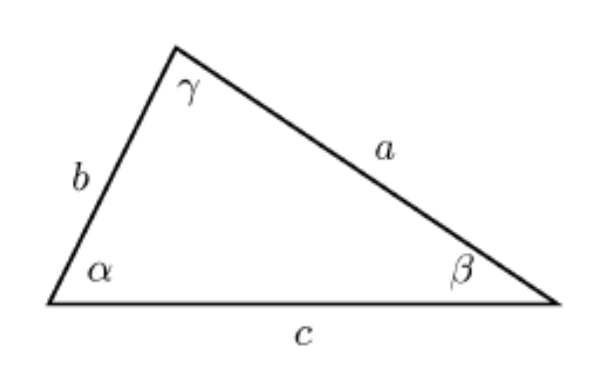
\includegraphics[width=0.5\textwidth]{fig2.1.png}
\end{center}

Fig. 1  Toate funcțiile trigonometrice sunt convexe (sau concave) dacă
argumentele lor sunt limitate la un domeniu adecvat și, în consecință,
există multe consecințe geometrice interesante ale inegalității lui Jensen.


Acum, dacă facem media acestor reprezentări ale ariei, vom obtine ca:
\begin{displaymath}
  \frac{1}{3}\left ( ab + ac + bc \right )= \left ( 2A \right )\frac{1}{3}\left \{ \frac{1}{sin \alpha } + \frac{1}{sin \beta } + \frac{1}{sin \gamma }\right \}, \label{eq:2.1} \tag{2.1}
\end{displaymath}
și aceasta este o formulă care ne conduce la a studia convexitatea functiei \(\frac{1}{sin x}\). Reprezentarea grafica a acesteia, \(x \mapsto \frac{1}{sin x}\), pentru \(x\in \left ( 0, \infty  \right )\) cu siguranță este convexă, iar presupunerea noastra pot fi confirmata prin calcularea derivatei a doua,
\begin{displaymath}
  {\left ( \frac{1}{sin x} \right )}''= \frac{1}{sin x} + 2\frac{cos^{2}x}{sin ^{3}x}> 0~~ \text{pentru orice}~~ x\in \left ( 0, \pi  \right )  \label{eq:2.2} \tag{2.2}
\end{displaymath}

	Prin urmare, din moment ce avem \[\frac{\left ( \alpha + \beta  + \gamma  \right )}{3}= \frac{\pi }{3},\] rezulta din inegalitatea lui Jensen ca
\begin{displaymath}
  \frac{1}{3}\left \{ \frac{1}{sin \alpha }  + \frac{1}{sin \beta } + \frac{1}{sin \gamma }\right \}\geq \frac{1}{sin \frac{\pi }{3}} =  \frac{2}{\sqrt{3}},
\end{displaymath}
deci, folosind inegalitatea \ref{eq:2.1}, obtinem estimarea ceruta
\begin{displaymath}
 \max \left ( ab, ac, bc \right )\geq \frac{1}{3}\left ( ab + ac + bc \right )\geq \frac{4}{\sqrt{3}}A. \label{eq:2.3} \tag{2.3}
\end{displaymath}

\end{proof}
\begin{remark}
Această problemă este strâns legată de o inegalitate binecunoscută a lui Weitzenböck care afirmă că în orice triunghi avem
\begin{displaymath}
  a^{2} + b^{2} + c^{2} \geq \frac{4}{\sqrt{3}}A. \label{eq:2.4} \tag{2.4}
\end{displaymath}

De fapt, pentru a trece de la inegalitatea \ref{eq:2.3} la inegalitatea lui Weitzenböck trebuie doar să ne amintim ca
\begin{displaymath}
  ab + ac + bc \leq a^{2} + b^{2} + c^{2},
\end{displaymath}
care este o inegalitate bine cunoscuta pe care o putem obtine in doua moduri  - folosind inegalitatea lui Cauchy sau golosind inegalitatea MA-MG

	Inegalitatea lui Weitzenböck se dovedește a avea multe demonstratii instructive - Engel (1998) a dat unsprezece!
Există câteva metode matematice pe care le-am putea numi generic "improvers"; în linii mari, acestea sunt metode care pot fi utilizate într-un mod algoritmic pentru a generaliza o identitate, sau pentru a îmbunătăți un rezultat dat.
\end{remark}
Următoarea problemă oferă un exemplu de alt fel. Aceasta sugerează cum am putea imbunatati aproape orice rezultat care a fost obtinut folosind inegalitatea lui Jensen

\begin{problem}
(Formula defectului a lui Hölder)

Daca \(f : \left [ a,b  \right ] \to \mathbb{R}\) este derivabila de doua ori si
\begin{displaymath}
  0 \leq m \leq  f''\left ( x \right ) \leq  M,~ pentru orice ~x\in \left [ a,b \right ], \label{eq:2.5} \tag{2.5}
\end{displaymath}
atunci pentru orice  \(a\leq x_{1}\leq x_{2}\leq ....\leq x_{n} \leq b \) si orice numere reale pozitive \(p_{k}, k= 1,2,.....,n \) cu \(p_{1} + p_{2} + \cdots+ p_{n} = 1\),  exista  \(\mu \in \left [ m, M \right ]\) pentru care are loc egalitatea
\begin{displaymath}
  \sum_{k = 1}^{n}p_{k}f\left ( x_{k} \right ) - f\left ( \sum_{k = 1}^{n} p_{k}x_{k}\right ) = \frac{1}{4}\mu \sum_{j = 1}^{n}\sum_{k = 1}^{n}p_{j}p_{k}\left ( x_{j} - x_{k} \right )^{2}. \label{eq:2.6} \tag{2.6}
\end{displaymath}
\end{problem}
\begin{remark}
Acest rezultat provine din aceeași lucrare faimoasă din 1885 a lui Otto Ludwig Hölder (1859 - 1937) în care se găseşte demonstratia inegalităţii care are a ajuns să fie cunoscută  ca ”inegalitatea lui Hölder”. Formula defectului \ref{eq:2.6} este mult mai puțin cunoscută, dar este totuși valoroasă. Aceasta oferă o măsură perfect naturală a diferenței dintre cele două părți ale inegalității lui Jensen și ne spune cum să învingem versiunea  inegalității lui Jensen ori de câte ori putem verifica ipoteza suplimentară \ref{eq:2.5}.
În mod similar, dacă M este mic, să spunem \(0 \leq M \leq \epsilon\), atunci inegalitatea \ref{eq:2.5} ne spune că f se comportă mai degrabă ca o funcție afină, \(f\left ( x \right ) = \alpha  + \beta x\). Pentru o funcție afină, partea stângă a egalitatii \ref{eq:2.6} este identic egal cu zero, dar în general, relatia \ref{eq:2.6} afirmă ceva mai subtil. Mai precis, ne spune că partea stângă este un mic multiplu al unei expresii  în care valorile \(x_{j}, j = 1,2,\cdots ,n \) sunt raspandite pe intreg intervalul \(\left [ a, b \right ]. \)
\end{remark}
\begin{proof}
Această problemă ne duce in mod firesc la urmatoarea intrebar: Cum putem folosi faptul că \(0\leq m\leq {f}''\left ( x \right )\leq M \)?

Odata ce ne-am pus aceasta intrebare, s-ar putea să nu fie nevoie de mult pentru a observa că cele două funcții
\begin{displaymath}
  g\left ( x \right ) = \frac{1}{2}Mx^{2} - f\left ( x \right )~~ si~~
h\left ( x \right ) = f\left ( x \right ) - \frac{1}{2}mx^{2}
\end{displaymath}
sunt doua functii convexe.
Aceasta observatie ne indeamna sa ne intrebam ce spune inegalitatea lui Jensen despre aceste functii.\\
Pentru \(g\left ( x \right )\), inegalitatea lui Jensen ne da marginirea
\begin{displaymath}
  \frac{1}{2}M\bar{x}^{2} - f\left ( \bar{x} \right )\leq \sum_{k = 1}^{n}p_{k}\left \{ \frac{1}{2}Mx_{k}^{2} - f\left ( x_{k} \right )\right \}
\end{displaymath}
unde am notat \(\bar{x} = p_{1}x_{1}+ p_{2}x_{2}+ \cdots + p_{n}x_{n}\) si aceasta inegalitate este usor de rearanjat  pentru a obtine
\begin{displaymath}
  \left \{ \sum_{k = 1}^{n} p_{k}f\left ( x_{k} \right )\right \} - f\left (\bar{x}  \right )\leq \frac{1}{2}M\left \{ \left ( \sum_{k=1}^{n} p_{k}x_{k}^{2}\right ) - \bar{x}^{2} \right \} = \frac{1}{2}M\sum_{k = 1}^{n}p_{k}\left ( x_{k} - \bar{x} \right )^{2}.
\end{displaymath}

Un calcul analog pentru  \(h\left ( x \right )\) ne ofera o limita inferioara
\begin{displaymath}
  \left \{ \sum_{k = 1}^{n} p_{k}f\left ( x_{k} \right )\right \} - f\left (\bar{x}  \right )\geq \frac{1}{2}m\sum_{k = 1}^{n}p_{k}\left ( x_{k} - \bar{x} \right )^{2}
\end{displaymath}
si aceste limite superioara si inferioara aproape completeaza demonstratia egalitatii  \ref{eq:2.5}. Singurul lucru care lipseste este identitatea
\begin{displaymath}
  \sum_{k = 1}^{n}p_{k}\left ( x_{k} - \bar{x} \right )^{2} = \frac{1}{2}\sum_{j = 1}^{n}\sum_{k = 1}^{n} p _{j}p_{k}\left ( x_{j} - x_{k} \right )^{2}
\end{displaymath}
care se poate verifica usor prin calcul direct folosind definitia lui \(\bar{x}\).
\end{proof}
Comvexitatea si inegalitatea lui Jensen ofera solutii simple pentru multe probleme.
	Urmatoarea problema vine din celebra sectiune cu probleme a ”American Mathematical Monthly” si ofera un exemplu clasic al acestei afirmatii.
	La inceput problema pare destul de usoara, dar, curand, intampinam dificultati.

\begin{problem}(AMM 2002, Proposed by M. Mazur)\\
Aratati ca daca a,b si c, sunt numere reale pozitive care verifica \(abc \geq 2^{9}\), atunci
\begin{displaymath}
  \frac{1}{\sqrt{1 + \left ( abc \right )^{\frac{1}{3}}}}\leq \frac{1}{3}\left \{ \frac{1}{\sqrt{1 + a}} + \frac{1}{\sqrt{1 + b}} + \frac{1}{\sqrt{1 + c}}\right \}    	
  \label{eq:2.7} \tag{2.7}
\end{displaymath}
\end{problem}
\begin{proof}
Media din partea dreaptă sugerează că inegalitatea lui Jensen s-ar putea dovedi utilă, în timp ce media geometrică din partea stângă sugerează că funcția exponențială va avea un rol.

Daca ne uitam mai atent, putem observa ca
\begin{displaymath}
  f\left ( x \right ) = \frac{1}{\sqrt{1+ e^{x}}}
\end{displaymath}
ne poate ajuta la folosirea inegalitatii lui Jensen. De fapt, odata ce am scris aceasta functie, se poate verifica aproape fara calcul ca inegalitatea propusa \ref{eq:2.7} este echivalenta cu
\begin{displaymath}
  f\left ( \frac{x + y + z}{3} \right )\leq \frac{1}{3}\left \{ f\left ( x \right ) + f\left ( y \right ) + f\left ( z \right ) \right \}    \label{eq:2.8} \tag{2.8}
\end{displaymath}
pentru orice $x, y, z$ astfel incat \(\exp\left ( x + y + z \right )\geq 2^{9}.\)

Pentru a vedea daca putem aplica inegalitatea lui Jensen, trebuie sa evaluam convexitatea lui f. Intr-adevar, avem

\begin{center}
	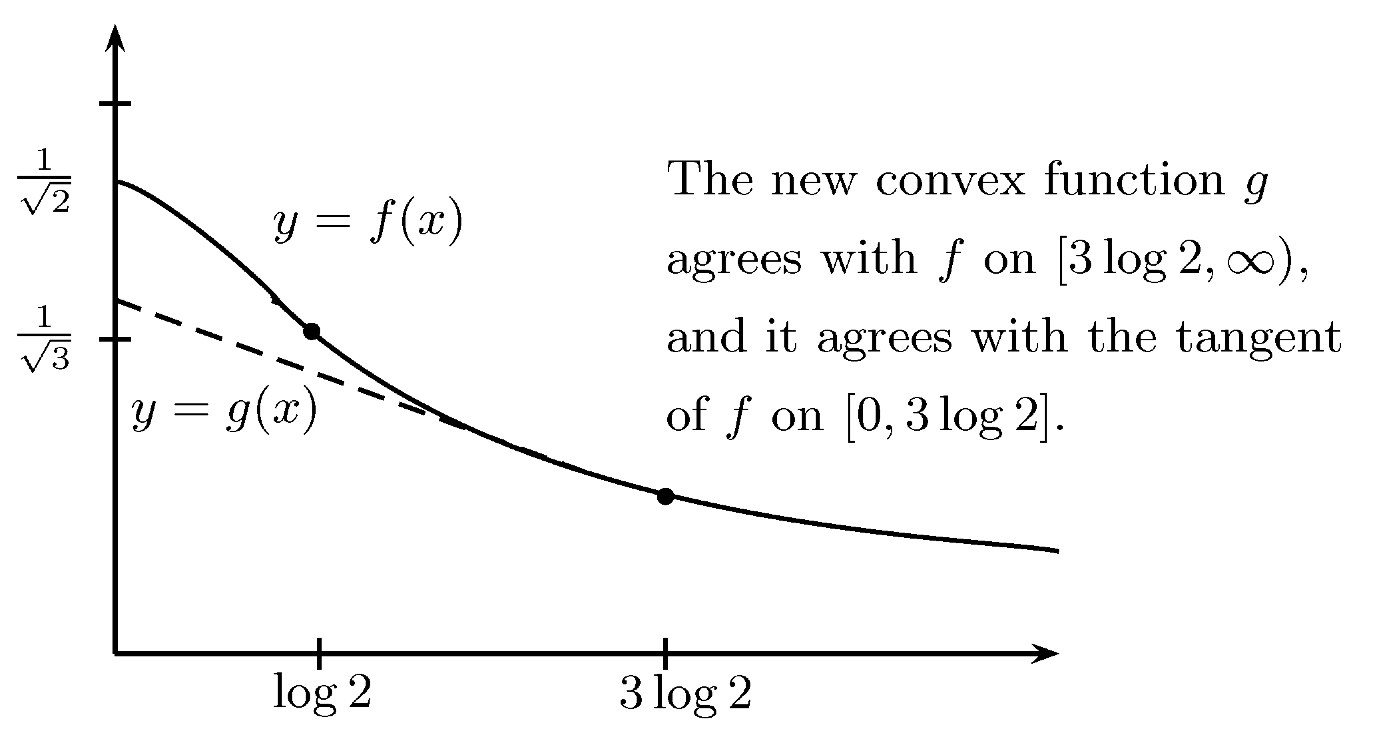
\includegraphics[width=1.0\textwidth]{fig_pb3.png}
\end{center}

\begin{displaymath}
  {f}'\left ( x \right ) = -\frac{e^{x}}{2 \left ( 1 + e^{x} \right )^{\frac{3}{2}}}
\end{displaymath}
si
\begin{displaymath}
  {f}''\left ( x \right ) = -\frac{1}{2}\left (  1 + e^{x} \right )^{-\frac{3}{2}}e^{x} + \frac{3}{4}\left ( 1 + e^{x} \right )^{-\frac{5}{2}}e^{2x}
\end{displaymath}

Cea de a doua egalitate ne arata ca\({f}''\left ( x \right ) \geq 0\) daca si numai daca avem \(e^{x}\geq 2\), atfel incat cu ajutorul inegalitatii lui Jensen  constatam ca inegalitatea initiala \ref{eq:2.8}  este adevarata cu conditia ca fiecare dintre termenii a, b si c sa fie mai mari sau egali cu2.

Dificultatea cu care ne confruntam aici este ca ipoteza problemei  ne spune doar  ca produsul \(abc\) rste mai mare sau egal cu \(2^{9}\); nu ni se da nicio  limita pentru termenii  individuali, cu exceptia faptului ca \( a > 0, b > 0 \) si \(c > 0\) . Astfel, inegalitatea lui Jensen nu poate completa demonstratia de la sine si noi trebuie să cautam alte informatii.

Exista multe idei pe care le-am putea incerca, dar inainte de a merge prea departe,  ar trebui sa luam in considerare graficul lui \(f\left ( x \right )\). Ceea ce  gasim  din graficul  reprezentat in Figura 3 este ca \(f\left ( x \right ) \) arata convexa pe interval \(\left [ 0, 10 \right ]  \), in ciuda faptului ca calculul care arata ca \(f\left ( x \right ) \) este concava pe \(\left [ 0, \log _{} 2\right ] \) si convexa pe \(\left [ \log _{} 2 , \infty \right ) \). Astfel, graficul nostru ofera o noua speranta; poate ca o mica modificare a lui \(f\) ar putea conduce la convexitatea de care noi avem nevoie pentru a rezolva problema.

Cand ne gandim la modul in care am sperat sa folosim \(f\) cu inegalitatea lui Jensen, in curand ne dăm seama ca ne putem ușura puțin sarcina. Sa presupunem, de exemplu, ca putem gasi o functie convexa \(g : \left [ 0 , \infty  \right ) \to \mathbb{R}\) astfel încât sa avem  conditiile:
\begin{displaymath}
  g\left ( x \right ) \leq  f\left ( x  \right ),~~ pentru~~ orice~~ x \in  \left [ 0 , \infty  \right )    \label{eq:2.9} \tag{2.9}
\end{displaymath}
si conditia complementara
\begin{displaymath}
  g \left ( x \right ) = f \left ( x \right ), ~~pentru~~ orice~~  x\geq 3 \log 2. \label{eq:2.10} \tag{2.10}
\end{displaymath}

Pentru o astfel de functie, inegalitatea lui Jensen ne spune  ca daca x,y si z verifica \[exp \left ( x + y + z \right )\geq  2^{9} \] avem inegalitatile
\begin{displaymath}
\begin{split}
  f\left ( \frac{x + y + z}{3} \right ) &= g\left ( \frac{x + y + z}{3} \right )\\
   &\leq  \frac{1}{3}\left \{ g\left ( x \right ) + g\left ( y \right ) + g\left ( z \right ) \right \} \leq  \frac{1}{3}\left \{ f\left ( x \right ) + f\left ( y \right ) + f\left ( z \right ) \right \}.
  \end{split}
\end{displaymath}

Primul și ultimul termen al acestei inegalitati conduc la inegalitatea \ref{eq:2.8}, deci soluția problemei ar fi completă, cu excepția unui mic detaliu — mai trebuie să arătăm că există o functie  g convexa pe \( \left [ 0 , \infty  \right ) \) astfel incat  \(g\left ( x \right ) \leq  f\left ( x \right )\) pentru orice  \(x \in \left [ 0 , 3\log 2 \right ]\) și \( f\left ( x \right ) = g\left ( x \right )\) pentru orice \( x \geq 3\log 2\).

O modalitate de a construi o funcție convexă \(g\) cu proprietățile  descrise mai sus este să luăm  \(g\left ( x \right ) = f\left ( x \right )\) pentru \(x \geq  3\log2\) și să definim \(g\left ( x \right )\) pe \(\left [ 0 , 3\log 2 \right ]\) prin extrapolare liniară. Astfel, pentru \(x\in \left [ 0 , 3\log 2 \right ]\), luăm
\begin{displaymath}
  g\left ( x \right ) - f\left ( 3\log 2 \right ) + \left ( x - 3\log 2 \right ){f}'\left ( 3\log2 \right ) = \frac{1}{3} + \left ( 3\log2 - x  \right )\left ( \frac{4}{27} \right )
\end{displaymath}

Trei observatii simple sunt acum suficiente pentru a demonstra ca \(g\left ( x \right )\leq f\left ( x \right )\), pentru orice \(x\geq 0\). Pentru inceput, pentru \(x\geq 3\log 2\), avem \(g\left ( x \right ) = f\left ( x \right )\) din definitie.

Cea de a doua observatie, pentru \(\log 2 \leq  x \leq  3\log 2\) avem  \(g( x )\leq f\left ( x \right ) \) pentru ca aici  \(g\left ( x \right )\) are valoarea unei drepte tangente la \((f\left ( x \right )\) si din convexitatea lui f pe \(\log 2 \leq  3 \leq 3\log 2\) dreapta tangenta este sub f.

Cea de a treia observatie, in regiunea critica \(0\leq  x \leq \log2\), avem \(g\left ( x \right ) \leq  f\left ( x \right )\) deoarece,
\begin{enumerate}
  \item f este concava,
  \item g este liniara,
  \item f este mai mare decat g la capetele intervalului \(\left [ 0 , \log 2 \right ]\).
\end{enumerate}
Mai precis, avem
\begin{displaymath}
  g\left ( 0 \right ) = 0.641\cdots \leq f\left ( 0 \right ) = \frac{1}{\sqrt{2}} = 0.707\cdots,
\end{displaymath}
in timp ce in cel de-al doilea punct avem
\begin{displaymath}
  g\left ( \log 2 \right ) = 0.538\cdots  \leq f\left ( \log2 \right ) = \frac{1}{\sqrt{3}} = 0.577\cdots.
\end{displaymath}

Astfel, functia convexa \(g\) este intr-adevar un minorant al functiei \(f\) care se afla in concordanta cu \(f\) pe \(\left [ 3\log 2 , \infty  \right )\), asadar rezolvarea problemei este completa.
\end{proof}
\begin{problem} (O inegalitate renascentista)\\
   Matematicianul renascentist Pietro Mengoli (1625 – 1686) a avut nevoie doar de algebra elementara pentru a demonstra inegalitatea
 \begin{displaymath}
   \frac{1}{x - 1} + \frac{1}{x} + \frac{1}{x + 1} > \frac{3}{x} , \text{pentru orice } x > 1, \label{eq:2.11} \tag{2.11}
 \end{displaymath}
totusi a obtinut o revendicare asupra numuririi intelectuale atunci cand a folosit asta pentru a oferi una dintre cele mai timpurii dovezi ale divergentei seriilor armonice,
\begin{displaymath}
  H_{n} = 1 + \frac{1}{2} + \frac{1}{3} + \cdots + \frac{1}{n} \Rightarrow \lim_{n \to \infty } H_{n} = \infty \label{eq:2.12} \tag{2.12}
\end{displaymath}

Redescoperiti demonstratia algebrica a inegalitatii lu Mengoli (2.4.1) si verificati faptul ca rezulta si din inegalitatea lui Jensen. Mai departe, aratati, cum a facut Mengoli, faptul ca inegalitatea \ref{eq:2.11} implica divergenta lui \(H_{n}\) .
\end{problem}
\begin{proof}
Simplificand \(\frac{1}{x}\) din ambele parti si adunand fractiile se vede ca inegalitatea lui Mengoli este echivalenta cu inegalitatea  triviala \(x^{2} >  x^{2} – 1\). \\
Pentru o demonstratie folosind inegalitatea lui Jensen, observam ca \(x \mapsto \frac{1}{x}\) este stict convexa. Aplicam inegalitatea lui Jensen pentru $x_1=x-1,$ $x_2=x,$ $x_3=x-1,$ si $\lambda_i=1/3,~i=1, 2, 3:$
\[
f\biggl(\frac{1}{3}(x-1+x+x+1)\biggr)=f(x)<\frac{1}{3}f(x+1)+\frac{1}{3}f(x)+\frac{1}{3}f(x-1)\Leftrightarrow
\]
\[
\frac{1}{x}<\frac{1}{3}\frac{1}{x+1}+\frac{1}{3}\frac{1}{x}+\frac{1}{3}\frac{1}{x-1}
\]
care inmultita cu trei este inegalitatea lui Mengoli.\\
In final, pentru o versiune moderna a demonstratiei lui Mengoli ca \(H_{n}\) diverge, presupunem prin absurd ca \(H_{\infty }< \infty\) si scriem \(H_{\infty }\) ca
\begin{displaymath}
  1 + \left ( \frac{1}{2} + \frac{1}{3} + \frac{1}{4} \right ) + \left ( \frac{1}{5} + \frac{1}{6} + \frac{1}{7} \right ) + \left ( \frac{1}{8} + \frac{1}{9} +\frac{1}{10} \right )+\cdots.
\end{displaymath}

Acum, prin aplicarea inegalitatii lui Mengoli in cadrul grupurilor formate gasim ca
\[
H_{\infty }>1 + \frac{3}{3} + \frac{3}{6} + \frac{3}{9} + ..= 1 + H_{\infty }
\]
care ne conduce la contradictia \(H_{\infty } > 1 + H_{\infty }\).
\end{proof}
\begin{remark}
Potrivit lui Havil, Mengoli a fost cel care a propus pentru prima data problema determinarii valorii sumei \[1 + \frac{1}{2^{2}} + \frac{1}{3^{2}} + \cdots.\]
Problema a rezistat eforturilor celor mai buni matematicieni ai Europei pana in anul 1731 cand L. Euler a determinat valoarea ca fiind \(\frac{\pi^{2}}{6}\).
\end{remark}

\begin{problem}
Aratati ca daca \(x , y , z > 0\) si \(x+ y + z = 1\), atunci
\begin{displaymath}
  64 < \left ( 1 + \frac{1}{x} \right )\left ( 1 + \frac{1}{y} \right )\left ( 1 + \frac{1}{z} \right ).
\end{displaymath}
\end{problem}
\begin{proof}
Inegalitatea rezulta prin aplicarea inegalitatii lui Jensen functiei
\begin{displaymath}
  f\left ( t \right ) = \ln \left ( 1+\frac{1}{t} \right ) = \ln \left ( 1 + t \right ) - \ln \left ( t \right ),~t>0
\end{displaymath}
care este strict convexa deoarece
\begin{displaymath}
  {f}''\left ( t \right ) = -\frac{1}{\left ( 1 + t \right )^{2}} + \frac{1}{t^{2}} > 0,  \text{pentru orice } t > 0.
\end{displaymath}

Intr-adevar, pentru pentru $x_1=x,$ $x_2=y,$ $x_3=z,$ si $\lambda_i=1/3,~i=1, 2, 3:$
\[
f\biggl(\frac{1}{3}(x+y+z)\biggr)=f\biggl(\frac{1}{3}\biggr)<\frac{1}{3}f(x)+\frac{1}{3}f(y)+\frac{1}{3}f(z)\Leftrightarrow
\]
\[
\ln (4)<\frac{1}{3}\ln\biggl(1+\frac{1}{x})\biggr) +\frac{1}{3}\ln\biggl(1+\frac{1}{y}\biggr)+\frac{1}{3}\ln\biggl(1+\frac{1}{z}\biggr)\Leftrightarrow
\]
\[
3\ln (4)< \ln\biggl((1+\frac{1}{x})(1+\frac{1}{y})(1+\frac{1}{z})\biggr)
\]
si aplicand exponentiala obtinem inegalitatea dorita.
\end{proof}


\begin{problem} (Inegalitatea ariei n-poligonului)

Figura 4 sugereaza ca  dintre toate poligoanele convexe cu n laturi care pot fi inscrise intr-un cerc, numai n-gonul regulat are aria maxima. Poate inegalitatea lui Jensen sa fie folosita pentru a confirma aceasta afirmatie?

\begin{center}
	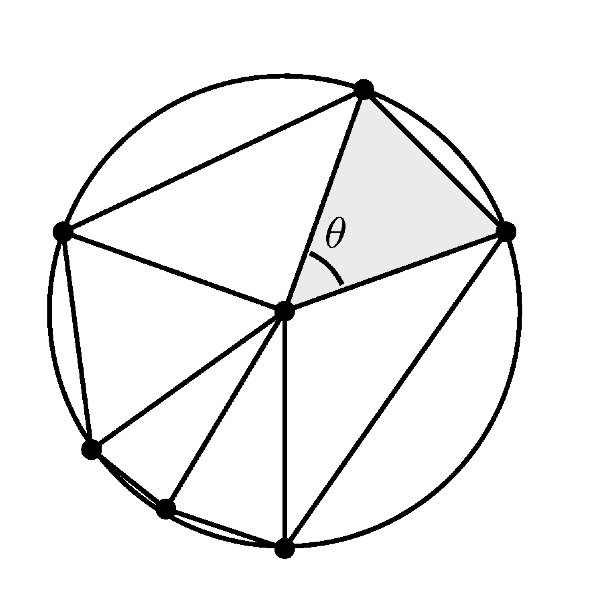
\includegraphics[width=0.5\textwidth]{fig_pb6.png}
	\\ Figura 4
\end{center}
\end{problem}
\begin{proof}
Din figura geometrica precizata, daca presupunem fara a restrange generalitatea ca raza cercului este 1, aria A a unui poligon inscris cu n laturi poate fi scrisa ca
\begin{displaymath}
  A = \frac{1}{2}\sum_{k = 1}^{n} \sin \theta _{k} ~~unde ~~0< \theta _{k} ~~si~~ \sum_{k = 1}^n{\theta _{k}} = 2\pi.
\end{displaymath}
	Cum functia  \(\sin \left ( \cdot  \right )\) este strict concava pe \(\left [ 0 , \pi  \right ]\), folosind inegalitatea lui Jensen avem
\begin{displaymath}
  A = \frac{1}{2}\sum_{k = 1}^{n} \sin \theta _{k}  \leq \frac{1}{2}n\sin\left ( \frac{1}{n}\sum_{k = 1}^{n}\theta _{k} \right ) = \frac{1}{2}n\sin \left ( \frac{2\pi }{n} \right ) = {A}'
\end{displaymath}
si avem egalitate daca si numai daca \(\theta _{k} = \frac{2\pi }{n}\) pentru orice \(1\leq k\leq n\). Cum \({A}'\) este aria unui n-poligon regulat inscris, optimalitatea presupusa este confirmata.
\end{proof}

\begin{problem} (Inegalitatile investitionale)

Daca \(0< r_{k} < \infty\). Daca investitia noastra de un dolar in anul \(k\) creste la \(1 +  r_{k}\) dolari la sfarsitul anului, numim \(r_{k}\) dobanda investitie in anul \(k\). Demonstrati ca valoarea
\begin{displaymath}
  V = \left ( 1 + r_{1} \right )\left ( 1 + r_{2} \right )\cdots \left ( 1 + r_{n} \right )
\end{displaymath}
a investitiei noastra dupa n ani verifica inegalitatile
\begin{displaymath}
  \left ( 1 + r_{G} \right )^{n} \leq \prod_{k = 1}^{n} \left ( 1 + r_{k} \right )\leq \left ( 1 + r_{A} \right )^{n}, \label{eq:2.13} \tag{2.13}
\end{displaymath}
unde
\begin{displaymath}
  r_{G} = \left ( r_{1}r_{2} \cdots r_{n}\right )^{\frac{1}{n}}~~ si~~ r_{A} = \frac{\left ( r_{1} + r_{2} +  \cdots+ r_{n}\right )}{n}.
\end{displaymath}
De asemenea explicati de ce aceaste inegalitati  pot fi vazuta ca un rafinament a inegalitatii MA-MG.
\end{problem}
\begin{proof}
Evident, inegalitatea din dreapta rezulta imediat daca aplicam inegalitatea MA-MG pentru
\begin{displaymath}
  a_{k} = 1 + r_{k},~ k =1,2,\cdots, n.
\end{displaymath}
Pentru inegalitatea din partea stanga aplicam inegalitatea lui Jensen aplicata functiei convexe
\[x \mapsto \ln\left ( 1 + e^{x} \right ).\]
Evident, daca notam cu $f$ aceasta functie, observam ca
\[
f''(x)=\frac{e^x}{(1+e^x)^2}>0,
\]
deci f este chiar strict convexa. Daca aplicam inegalitatea lui Jensen acestei functii pentru
\[
x_1=\ln r_1,\cdots, x_1=\ln r_1,~~\lambda_1=\frac{1}{n},\cdots, \lambda_n=\frac{1}{n},
\]
deducem si inegalitatea din stanga.\\
La final, daca extragem radacina de ordinul n si scadem 1, in toti termenii, vom vedea ca inegalitatea \ref{eq:2.13} rafineaza limita MA-MG,  \(r_{G} \leq r_{A}\) prin intercalarea termenului \(V^{\frac{1}{n}} – 1\) intre cele doua.
\end{proof}

\begin{problem} (Supraaditivitatea mediei geometrice)
	
Daca \(a_{j}\geq 0 \) si \(b_{j}\geq 0, j = 1 , 2, \cdots, n,\) atunci:
\begin{displaymath}
  \left ( a_{1}a_{2}\cdots a_{n} \right )^{\frac{1}{n}} + \left ( b_{1}b_{2}\cdots b_{n} \right )^{\frac{1}{n}} \leq  \left \{ \left ( a_{1} + b_{1}\right ) \left ( a_{2} + b_{2} \right )\cdots \left ( a_{n} + b_{n} \right )\right \}^{\frac{1}{n}}.
\end{displaymath}
\end{problem}
	\begin{proof}
	Pentru a construi o demonstratie cu ajutorul inegalitatii lui Jensen, mai intai impartim la
\(\left ( a_{1}a_{2}\cdots a_{n} \right )^{\frac{1}{n}}\) si notam \(c_{k}=\frac{b_{k}}{a_{k}},~k=1,\cdots, n\) deci inegalitatea de la care am pornit devine
\begin{displaymath}
  1 + \left ( c_{1}c_{2} \cdots c_{k}\right )^{\frac{1}{n}}\leq \left \{ \left ( 1 + c_{1} \right )\left ( 1 + c_{2} \right )\cdots \left ( 1 + c_{n} \right ) \right \}^{\frac{1}{n}}.
\end{displaymath}

Acum, daca scriem \(c_{j}\) ca \(exp\left (d _{j} \right )\), vom vedea ca obtinem forma echivalenta
\begin{displaymath}
  \ln\left ( 1 + exp\left ( \bar{d} \right ) \right ) \leq \frac{1}{n}\sum_{j = 1}^{n}\ln\left ( 1 + exp\left ( d_{j} \right ) \right ),
\end{displaymath}
unde
\begin{displaymath}
  \bar{d} = \frac{\left ( d_{1} + d_{2}  + \cdots + d_{n}\right )}{n}.
\end{displaymath}
Obsevam acum ca ultima inegalitate este pur si simplu inegalitatea lui Jensen pentru functia convexa \(x \mapsto \log \left ( 1 + e^{x} \right )\), astfel, rezolvarea este completa.
\end{proof}
\begin{remark}
O caracteristica a acestei solutii care merita remarcata este aceea ca progresul in rezolvarea problemei a venit rapid dupa ce impartirea a redus numarul de variabile de la \(2n\) la \(n\). Acest fenomen este de fapt destul de comun si astfel de reduceri merita aproape intotdeauna incercate.
\end{remark}

\begin{problem} (Technica lui Cauchy si Inegalitatea lui Jensen)

In 1906, J. L. W. V. Jensen a scris un articol care a fost inspirat de demonstratia data de Cauchy pentru inegalitatea MA-MG si, intr-un efort de a ajunge la miezul argumentului lui Cauchy, Jensen a introdus clasa de functii care satisfac inegalitatea
\begin{displaymath}
  f\left ( \frac{x + y}{2} \right ) \leq \frac{f\left ( x \right ) + f\left ( y \right )}{2} \text{pentru orice } x,y \in \left [ a, b \right ]. \label{eq:2.14} \tag{2.14}
\end{displaymath}

Astfel de functii sunt acum numite functii J-convexe si, dupa cum observam mai jos in problema care urmeaza, ele sunt doar putin mai generale decat functiie convexe definite de conditia
\begin{displaymath}
  f\left ( px + \left ( 1 - p \right )y \right )\leq pf\left ( x \right ) + \left ( 1-p \right )f\left ( y \right ).
\end{displaymath}

Sa se arate ca orice functie  J-convexa verifica inegalitatea
\begin{displaymath}
  f\left ( \frac{1}{n} \sum_{k = 1}^{n}x_{k}\right )\leq \frac{1}{n}\sum_{k = 1}^{n}f\left ( x_{k} \right )
\end{displaymath}
pentru orice
\begin{displaymath}
  \left \{ x_{k}: 1\leq k \leq n \right \} \subset \left [ a, b \right ]. \label{eq:2.15} \tag{2.15}
\end{displaymath}
\end{problem}
\begin{proof}
Vom aplica thenica pe care Cauchy a folosit-o pentru a demonstra inegalitatea mediilor. Astfel, pentru incepui presupunem ca \(n = 2^{k}, k=1,2,….,\) si demonstram \ref{eq:2.15} in acest caz.

Intr-adevar, daca luam in \ref{eq:2.14} $x=(x_1+x_2)/2$ si $y=(x_3+x_4)/2$ vom obtine ca
\begin{equation*}
  f\left ( \frac{x_1 + x_2+x_3+x_4}{4} \right ) \leq \frac{f\left ( \frac{x_1 + x_2}{2} \right) + f\left(\frac{x_3 + x_4}{2} \right )}{2} \leq
\end{equation*}
\begin{equation*}
   \frac{f\left (x_1) + f\left (x_2 \right )+f\left (x_3 \right )+f\left (x_4 \right ) \right)}{4} \text{pentru orice } x_1, \cdots, x_4 \in \left [ a, b \right ]\leq
\end{equation*}
Repetand procedeul obtinem \ref{eq:2.15} pentru orice $n=2^k,~k\geq 1.$\\
 Pentru a demonstra acum in cazul in care $n$ nu e de forma anterioara, alegem  \(k\) astfel incat \(n< 2^{k}\) si aplicam rezultatul pentru \(2^{k}\) sirului de valori \(y_{j} , 1\leq j\leq 2^{k}\) luand \(y_{j} = x_{j}\) pentru \(1\leq j\leq n \) si \(y_{j} = \frac{\left ( x_{1} + x_{2} + ....+ x_{n} \right )}{n}=\overline{x}\) pentru \(n< j\leq 2^{k}\), astfel vom avea
 \[
   f\left ( \frac{x_1 + \cdots+x_n}{2^k}+\frac{x}{2^k}+\cdots+\frac{x}{2^k} \right )=f\left( \frac{n \overline{x}}{2^k}+\frac{(2^k-n) \overline{x}}{2^k}\right)=f(\overline{x}) \leq
 \]
 \[
\frac{ f(x_1)}{2^k}+\cdots+\frac{ f(x_n)}{2^k}+\frac{(2^k-n)}{2^k}f(\overline{x})=\frac{ f(x_1)}{2^k}+\cdots+\frac{ f(x_n)}{2^k}+ (1-\frac{n}{2^k})f(\overline{x})
 \]
 care va implica
 \[
 f(\overline{x})=  f\left ( \frac{x_1 + \cdots+x_n}{n} \right )\leq f\left ( \frac{x_1}{n} \right )+\cdots+f\left ( \frac{x_n}{n} \right ),
 \]
 adica inegalitatea \ref{eq:2.15}.
\end{proof}

\begin{problem}  (Convexitatea si J-Convexitatea)

Demonstrati ca daca \(f : \left [ a,b \right ]\rightarrow \mathbb{R} \) este continua si J-convexa, atunci \(f\) trebuie sa fie convexa, adica pentru orice $x, y\in [a,b],~ p\in [0,1]$
\begin{displaymath}
  f\left ( px + \left ( 1 - p \right )y \right )\leq pf\left ( x \right ) + \left ( 1-p \right )f\left ( y \right.
\end{displaymath}
\end{problem}
\begin{remark}
Ca o curiozitatea, ar trebui sa punctam faptul ca exista functii J-convexe care nu sunt convexe. Cu toate acestea, astfel de functii sunt discontinue si foarte rar utilizate.
\end{remark}
\begin{proof}
Dupa cum am observat in solutia anterioara, avem ca pentru orice \(k = 1,2,\cdots\) are loc inegalitatea
\begin{displaymath}
  f\left ( \frac{1}{2^{k}} \sum_{j = 1}^{2^{k}}x_{j}\right ) \leq  \frac{1}{2^{k}}\sum_{j = 1}^{2^{k}}f\left ( x_{j}\right ),
\end{displaymath}
deci luand \(x_{j} = x\) pentru \(1\leq j\leq m\) si \(x_{j} = y\) pentru \(m< j\leq 2^{k}\) avem de asemenea
\begin{displaymath}
  f\left ( \left ( \frac{m}{2^{k}} \right )x + \left ( 1 - \frac{m}{2^{k}} \right )y \right )\leq \left ( \frac{m}{2^{k}} \right )f\left ( x \right ) + \left ( 1 - \frac{m}{2^{k}} \right )f\left ( y \right ).
\end{displaymath}
Daca alegem acum \(m_{t}\) si \(k_{t}\) astfel incat \(\frac{m_{t}}{2^{k_{t}}} \rightarrow p\) pentru \(t \rightarrow \infty\), atunci continuitatea lui f si inegalitatea precedenta vor implica
\begin{displaymath}
  f\left ( px + \left ( 1 - p \right )y \right ) \leq  pf\left ( x \right ) + \left ( 1 - p \right )f\left ( y \right ).
\end{displaymath}
\end{proof}

\begin{problem}
	Aratati ca pentru orice \(0\leq x , y , z \leq 1\), una are limita
\begin{displaymath}
  L\left ( x , y , z \right ) = \frac{x^{2}}{1 + y} + \frac{y^{2}}{1 + z} + \frac{z^{2}}{1 + x+ y} + x^{2} \left ( y^{2} - 1 \right )\left ( z^{2} - 1 \right ) \leq 2.
\end{displaymath}
\end{problem}
\begin{proof}
Functia \(L\left ( x,y,\ \right )\) este convexa in fiecare din cele trei variabile ale sale separat si prin argumentul detaliat mai jos, acest lucru implica faptul ca L trebuie sa atinga punctul maxim  in unul dintre varfurile cubului.

Dupa opt evaluari usoare constatam ca \(L \left ( 1,0,0 \right ) = 2\) si ca in niciun alt colt al cubului $[0, 1]^3$ L nu are o valoare mai mare, deci solutia va fi completa. Este de asemenea usor sa aratam ca daca o functie definita pe cub este convexa in fiecare variabila separat, atunci functia trebuie sa atinga maximul in unul dintre varfuri.

In primul rand se observa ca o functie convexa pe \(\left [ 0 , 1 \right ]\) trebuie sa isi atinga maximul in unul dintre punctele finale ale intervalului, deci, pentru orice valoare fixa dintre y si z, avem inegalitatea
\begin{displaymath}
  L\left ( x,y,z \right )\leq max \left \{ L\left ( 0,y,z \right ), L\left ( 1,y,z \right ) \right \}.
\end{displaymath}

 Similar din convexitatea lui \(y \mapsto L\left ( 0,y,z \right )\) si \(y \mapsto L\left ( 1,y,z \right )\)  rezulta ca \(L\left ( 0, y, z \right )\) este marginit superior de  \[\max \{L\left ( 0,0,z \right ), L\left ( 0,1,z \right )\}\] si \( L\left ( 1,y,z \right )\) este marginit superior de \[\max \{\left \{ L\left ( 1,0,z \right ) , L \left ( 1,1,z \right )\right \}\}.\]

 Luand toate aceste marginiri superioare, avem pentru orice valoare a lui z ca \(L\left ( x,y,z \right )\) este marginita de
 \[\max\left \{ L\left ( 0,0,z \right ), L\left ( 0,1,z \right ), L\left ( 1,1,z \right ) \right \}.\]

 Convexitatea lui \(z \mapsto L\left ( x,y,z \right )\) aplicata de patru ori ne da apoi marginirea
 \begin{displaymath}
  L\left ( x,y,z \right ) \leq  \max \left \{ L\left ( e_{1} , e_{2}, e_{3}\right ): e_{k}  = 0 \text{sau } e_{k} = 1 ~\text{pentru }~ k = 1,2,3\right \}
\end{displaymath}
\end{proof}


\begin{problem}
Pentru orice triunghi, teorema cosinusului care ne spune ca
\begin{displaymath}
  a^{2} = b^{2}+ c^{2} - abc\cos\alpha.
\end{displaymath}
Aratati ca aceasta teorema implica formula ariei
\begin{displaymath}
  a^{2} = \left ( b - c^{2} \right ) + 4 A\tan \left ( \frac{\alpha }{2} \right ),
\end{displaymath}
apoi aratati cum implica inegalitatea lui Jensen faptul ca in orice triunghi
\begin{displaymath}
  a^{2} + b^{2} + c^{2} \geq  \left ( a - b  \right )^{2} + \left ( b- c  \right )^{2} + \left ( c - a \right )^{2} + 4\sqrt{3}A.
\end{displaymath}
\end{problem}
\begin{proof}
Aceasta inegalitate este cunoscuta ca inegalitatea Hadwiger-Finsler , si furnizeaza una din cele mai frumoase rafinamente ale inegalitatii Weitzenböck.

Pentru a demonstra prima formula, observam ca
\begin{displaymath}
  a^{2} = b^{2} + c^{2} - 2ac\cos\alpha  = \left (  b - c \right )^{2} + 2bc\left ( 1 - \cos\alpha  \right )=
\end{displaymath}
\begin{displaymath}
 \left ( b - c \right )^{2} + \frac{4A\left ( 1 - \cos  \right )}{\sin \alpha } = \left ( b - c \right )^{2} + 4A\tan\left ( \frac{\alpha }{2} \right ),
\end{displaymath}
deci, prin simetrie si adunare, vedem ca
\(a^{2} + b^{2} + c^{2}\) este egal cu
\begin{displaymath}
  \left ( a - b  \right )^{2} + \left ( b - c \right )^{2} + \left ( c - a  \right )^{2} + 4A\left ( \tan\left ( \frac{\alpha }{2} \right ) + \tan\left ( \frac{\beta }{2} \right ) + \tan \frac{\gamma }{2} \right ).
\end{displaymath}
	Cum \(x \mapsto \tan x\) este convexa pe \(\left [ 0 , \frac{\pi }{2} \right ]\), inegalitatea lui Jensen implica
\begin{displaymath}
  \frac{1}{3}\left \{ \tan \left ( \frac{\alpha }{2} \right ) + \tan \left ( \frac{\beta }{2} \right )  + \tan \left ( \frac{\gamma }{2} \right )\right \} \geq  \tan\left ( \frac{\alpha  + \beta  + \gamma }{6} \right ) = \tan \left ( \frac{\pi }{6} \right)
\end{displaymath}

Si cum\(\tan \left ( \frac{\pi }{6} \right ) = \sqrt{3}\),  am incheiat demonstratia.
\end{proof}

\begin{problem} (Criteriul derivatei secunde si Teorema lui Rolle)
	
Este cunoscut faptul ca daca \({f}'' \geq 0\) pentru orice \(x\in \left [ a,b \right ]\), atunci \(f\) este convexa pe \(\left [ a,b \right ]\). Acest exercitiu schiteaza cum se poate demonstra acest lucru important prin estimarea diferentei
\begin{displaymath}
  f\left ( px_{1} + qx_{2}\right ) - pf\left ( x_{1} \right ) - qf\left ( x_{2} \right ).
\end{displaymath}
 prin compararea cu un polinom.
 \begin{enumerate}[a)]
\item Luam \(0< p < 1, q = 1-p\) si notam \(mu = px_{1} + px_{2}\) unde \(x_{1} < x_{2}\).  Gasiti polinomul patratic unic \(Q\left ( x \right )\) astfel incat  \(Q\left ( x_{1} \right ) = f\left ( x_{1} \right ), Q\left ( x_{2} \right ) = f\left ( x_{2} \right )\) si \(Q\left ( \mu  \right ) = f\left ( \mu  \right )\).
\item Folosind faptul ca \(\Delta \left ( x \right ) =  f\left ( x \right ) - Q\left ( x \right )\) are trei zerouri distincte in \(\left [ a,b \right ]\) pentru a demosntra ca exista un \(x^{*}\) astfel incat \({\Delta }''\left ( x^{*} \right ) = 0\).
\item In final, explicati cum \({f}''\left ( x \right ) \geq 0\) pentru orice \(x\in \left [ a,b \right ]\) si \({\Delta }''\left ( x^{*} \right ) = 0\) implica faptul ca \(f\left ( px_{1} + qx_{2} \right ) - pf\left ( x_{1} \right ) - qf\left ( x_{2} \right ) \geq 0\).
\end{enumerate}
\end{problem}
\begin{proof}
Polinomul \(Q\left ( x \right )\) poate fi scris astfel:
\begin{displaymath}
  \frac{\left ( x - x_{2} \right )\left ( x - \mu  \right )}{\left ( x_{1}  - x_{2}\right )\left ( x_{1} - \mu  \right )} f\left ( x_{1} \right ) + \frac{\left ( x - x_{1} \right )\left ( x - \mu  \right )}{\left ( x_{2}  - x_{1}\right )\left ( x_{2} - \mu  \right )}  f\left ( x_{2} \right ) +  \frac{\left ( x - x_{1} \right )\left ( x - x_{2}  \right )}{\left ( \mu   - x_{1}\right )\left (  \mu - x_{2} \right )}f\left ( \mu \right ).
\end{displaymath}
Dupa ce plicam Teorem lui Rolle de doua ori observam faptul ca  \({Q}'\left ( x \right ) - {f}'\left ( x \right )\) are un zero in \(\left ( x_{1} , \mu \right )\) si un alt zero in \(\left ( \mu  , x_{2} \right )\), deci o a treia aplicare a Teoremei lui Rolle ne arata ca exista un \(x^{*}\) intre aceste zerouri pentru care avem \(0 = {Q}''\left ( x \right ) - {f}''\left ( x^{*} \right )\). Prin urmare o sa avem \({Q}''\left ( x^{*}  \right ) = {f}''\left ( x^{*} \right )\geq 0\). Dar
\begin{displaymath}
  {Q}''\left ( x^{*}  \right ) = \frac{2f\left ( x_{1} \right )}{\left ( x_{1} - x_{2} \right )\left ( x_{1} - \mu  \right )} +  \frac{2f\left ( x_{2} \right )}{\left ( x_{2} - x_{1} \right )\left ( x_{2} - \mu  \right )} +  \frac{2f\left (\mu  \right )}{\left ( \mu  - x_{1} \right )\left ( \mu  - x_{2} \right )}
\end{displaymath}
Deci, luand
\begin{displaymath}
  p = \frac{\left ( x_{2} - \mu  \right )}{\left ( x_{2} - x_{1}\right )}
\end{displaymath}
si
\begin{displaymath}
  q = \frac{\left ( \mu  - x_{1} \right )}{\left ( x_{2} - x_{1} \right )}
\end{displaymath}
si simplificand, se constata ca ultima inegalitate se reduce la definitia convexitatii lui f.
\end{proof}
\begin{problem} (Transformare pentru obtinerea convexitatii)
Aratati ca pentru numere pozitive \(a , b si c\) care verifica \(a + b = c = abc\), avem
\begin{displaymath}
  \frac{1}{\sqrt{1 + a^{2}}} + \frac{1}{\sqrt{1 + b^{2}}} + \frac{1}{\sqrt{1 + c^{2}}} \leq \frac{3}{2}
\end{displaymath}
\end{problem}
\begin{proof}
Aceasta problema data la Olimpiada Nationala din Koreea in 1998 nu este usoara, chiar si cu indicatia oferita de titlul exercitiului. Cineva, care este norocos, poate stabili o legatura intre  ipoteza \(a + b + c = abc\) si binecunoscutul lucru ca intr-un triunghi, cu notatiile  ca in figura Fig 1
 avem
 \begin{displaymath}
   \tan\left ( \alpha  \right ) + \tan\left ( \beta   \right ) + \tan\left ( \gamma   \right ) = \tan\left ( \alpha  \right )\tan\left ( \beta   \right )\tan\left ( \gamma   \right ).
 \end{displaymath}
Aceasta identitate este usor de verificat tinand cont de faptul ca avem egalitatea \[\gamma  = \pi  - \left ( \alpha  - \beta  \right ),\] dar este cu siguranta mai usor sa ne amintim acest lucru decat sa descoperim pe loc.

Avand in vedere indiciul, evident vom lua in considerare variabilele,  \[\alpha  = \tan^{-1}\left ( a \right ),~ \beta = \tan ^{-1}\left ( b \right ),~\gamma  = \tan ^{-1}\left ( c \right ).\]
Conditiile \(a> 0\), \(b> 0\), \(c> 0\), si \(a+b+c = abc\) ne arata faptul ca \[\alpha > 0 ~\beta > 0~\gamma > 0~\alpha + \beta + \gamma  = \pi.\] Inegalitatea din enunt devine de asemenea \[\cos \alpha  + \cos \beta  + \cos \gamma  \leq \frac{3}{2}\] si acest lucru rezulta direct din Inegalitatea lui Jensen  tinand cont de  concavitatea functiei cos
 pe \(\left [ 0 , \pi  \right ]\)  si de egalitatea \(\cos \left ( \frac{\pi }{3} \right ) = \frac{1}{2}\).
\end{proof}
\begin{problem} (Teorema Gauss-Lucas)
Sa se arate ca pentru orice polinom complex \(P\left ( z \right ) = a_{0} + a_{1}z + ..... +a_{n}z^{n}\) radacinile derivatei \({P}'\left ( z \right )\) sunt cuprinse in acoperirea convexa \(H\) a radacinilor lui \(P\left ( z \right )\).
\end{problem}
\begin{proof}
Daca scriem
\begin{displaymath}
  P\left ( z \right ) = a_{n}\left ( z - r_{1} \right )^{m_{1}}\left ( z - r_{2} \right )^{m_{2}}\cdots \left ( z - r_{n} \right )^{m_{k}},
\end{displaymath}
unde  \(r_{1} , r_{2}, \cdots, r_{k}\) sunt radacinile distincte ale lui \(P\left ( z \right )\) si \(m_{1} , m_{2}, \cdots, m_{k}\) sunt multiplicitatile corespunzatoare si impartim \({P}'\left ( z \right )\) la \( P\left ( z \right )\)obtinem
\begin{displaymath}
  \frac{{P}'\left ( z \right ) }{P\left ( z \right )} = \frac{m_{1}}{z - r_{1}} + \frac{m_{2}}{z - r_{2}}+ \cdots + \frac{m_{k}}{z - r_{n}} .
\end{displaymath}
Acum daca \(z_{0}\) este o radacina a lui \({P}'\left ( z \right )\) care este de asemenea o radacina a lui \(P\left ( z \right )\), atunci \(z_{0}\) este automat in \(H\) , deci fara a reduce generalitatea, putem presupune ca \(z_{0}\)  este o radacina a lui  \({P}'\left ( z \right )\) care nu este o radacina a lui \(P\left ( z \right )\), caz in care gasim
\begin{displaymath}
  0 = \frac{m_{1}}{z_{0} - r_{1}} + \frac{m_{2}}{z_{0} - r_{2}} +\cdots+ \frac{m_{k}}{z_{0} - r_{k}}
\end{displaymath}
\begin{displaymath}
= \frac{m_{1}\left (\bar{z_{0}} - \bar{r_{1}}\right )}{\left | z_{0}  - r_{1}\right |^{2}} + \frac{m_{2}\left (\bar{z_{0}} - \bar{r_{2}}\right )}{\left | z_{0}  - r_{2}\right |^{2}} + \cdots+ \frac{m_{k}\left (\bar{z_{0}} - \bar{r_{k}}\right )}{\left | z_{0}  - r_{k}\right |^{2}}.
\end{displaymath}
Daca luam
\begin{displaymath}
  \omega _{k} =\frac{ m_{k}}{\left | z_{0}  - r_{k}\right |^{2}},
\end{displaymath} atunci putem scrie aceasta identitate ca
\begin{displaymath}
  z_{0} = \frac{\omega _{1}r_{1} +\omega _{2}r{_2}+\cdots+ \omega _{k}r{_k} }{\omega _{1} + \omega _{2} + \cdots + \omega _{k}},
\end{displaymath}
care ne arata ca \(z_{0}\) este o combinatie convexa a radacinilor lui \(P\left ( z \right )\).
\end{proof}

\begin{problem} (Inegalitatea lui Wilf)

Aratati ca daca \(H\) este acoperira convexa a radacinilor polinomului complex \(P = a_{0} + a_{1}z + ..... +a_{n}z^{n}\), atunci avem
\begin{displaymath}
  \left | \frac{a_{n}}{P\left ( z \right )} \right |^{\frac{1}{n}}\leq \frac{1}n\cos{\psi }\left | \frac{{P}'\left ( z \right )}{P\left ( z \right )} \right | , \text{pentru orice } z\notin H, \label{eq:2.16} \tag{2.16}
\end{displaymath}
unde unghiul \(\psi\) este definit de figura Fig 5. Aceasta inegalitate ne ofera in acelasi timp si o noua dovada si o rafinare cantitativa  a Teoremei clasice Gauss- Lucas de la problema anterioara.
\begin{center}
	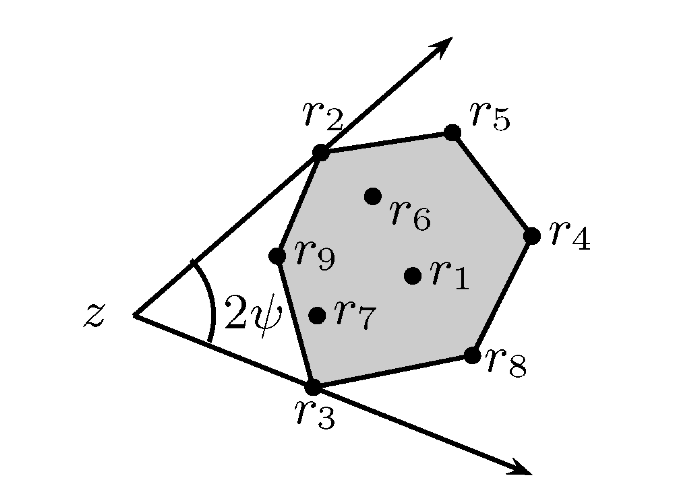
\includegraphics[width=0.5\textwidth]{fig_pb14.png}
	\\ Figura 5
\end{center}
Figura 5  Unghiul de vizualizare \(2\psi\) al acoperirii convexe a multimii radacinilor \(r_{1} , r_{2} , \cdots, r_{n}\)  lui \(P\left ( z \right )\), determina parametrul \(\psi\) pe care il gasim in rafinarea cantitativa a lui Wilf a Teoremei Gauss-Lucas.
\end{problem}
\begin{proof}
Scriem \(r_{1} , r_{2} ,\cdots,r_{n}\) radacinile lui \(P\) repetate in functie de multiplicitatea lor si pentru un \(z\) care se afla in afara acoperirii convexe \(H\) scriem \(z - r_{j}\) in forma polara \(z - r_{j} = \rho _{j}e^{i\theta j}\). Atunci avem
\begin{displaymath}
  \frac{1}{z - r_{j}} = \rho _{j}^{-1}e^{-\theta ji} , 1 \leq  j \leq  n,
\end{displaymath}
si diferenta intre argumentele \(\theta _{j}, 1 \leq j\leq n\) este mai mica sau egala cu \(2\psi\). Astfel, din Inegalitatea  MA-MG forma complexa,avem
\begin{displaymath}
  \left ( \cos\psi  \right )\left | \frac{1}{z - r_{1}} \frac{1}{z - r_{2}}\cdots \frac{1}{z - r_{n}} \right|^{\frac{1}{n}} \leq  \frac{1}{n} \left | \sum_{j = 1}^{n}\frac{1}{z - r_{j}} \right |
\end{displaymath}
care in termeni de \(P\) si \({P}'\), se scrie ca
\begin{displaymath}
   \left | \frac{a_{n}}{P\left ( z \right )} \right |^{\frac{1}{n}}\leq \frac{1}{n\cos\psi }\left | \frac{{P}'\left ( z \right )}{P\left ( z \right )} \right |,  \text{pentru orice }z \notin H,
\end{displaymath}
 ceea ce doream sa demonstram.
\end{proof}

\begin{problem}
Daca toate radacinile polinomului \(P\left ( z \right ) = a_{n}z^{n} +\cdots +a_{1}z + a_{0}\) sunt continute in discul unitate \(U= \left \{ z: \left | z \right |\leq 1 \right \}\), atunci
\begin{displaymath}
    n\left | a_{n} \right |^{\frac{1}{n}}\left | P\left ( z \right ) \right |^{\frac{\left ( n-1 \right )}{n}}\sqrt{1 - \left | z \right |^{-2}}\leq \left | {P}'\left ( z \right ) \right |, \text{pentru orice } z\notin U. \label{eq:2.17} \tag{2.17}
\end{displaymath}
\end{problem}
\begin{proof}
Daca \(2\psi\) este unghiul de vizualizare determinat de \(U\) cand este privit din \(z \notin U\), atunci avem \(1 = \left | z \right |\sin\psi\), deci Teorema lui Pitagora ne spune ca \(\cos\psi = \left ( 1 - \left | z \right |^{-2} \right )^{\frac{1}{2}}\). Inegalitatea  \ref{eq:2.17} rezulta apoi direct din inegalitatea lui Wilf, \ref{eq:2.16}.
\end{proof}
\begin{problem}
Aratati ca daca \(0 < r < 1\) si daca numerele complexe \(z_{1}, z_{2},...,z_{n}\) sunt in discul \(D = \left \{ z: \left | z \right | \leq r\right \}\), atunci exista \(z_{0} \in D\) astfel incat
\begin{displaymath}
    \prod_{j = 1}^{n}\left ( 1 + z_{j} \right ) = \left ( 1 + z_{0} \right )^{n}.\label{eq:2.18} \tag{2.18}
\end{displaymath}
\end{problem}
\begin{proof}
Discul \(D_{0} = \left \{ z : \left | 1 - z \right |\leq 1 \right \}\) scris in coordonate polare este
\begin{displaymath}
    \left \{ re^{i\theta }: 0 \leq r\leq 2\cos\theta , -\frac{\pi }{2}< \theta  < \frac{\pi }{2} \right \},
\end{displaymath}
deci pentru fiecare \(j\) putem scrie \(1 + z_{j}\) ca \(r_{j}e^{i\theta _{j}}\) unde \[-\frac{\pi }{2}< \theta  < \frac{\pi }{2},~r_{j}\leq 2\cos\theta _{j}.\]
 Rezulta imediat ca \[z_{0} = -1 + \left ( r_{1} r_{2}\cdots r_{n}\right )^{\frac{1}{n}}exp\left ( i\frac{\left ( \theta _{1} + \theta _{2} +....+ \theta _{n} \right )}{n} \right )\] este solutia ecuatiei lui Nievergelt \ref{eq:2.18} si pentru a demonstra ca \(z_{0}\in D \)este suficient sa aratam ca \(1 + z_{0}\in D_{0}\), echivalent, trebuie sa aratam ca
\begin{displaymath}
    \left ( r_{1} r_{2} \cdots r_{n}\right )^{\frac{1}{n}}\leq 2\cos\left ( \frac{\theta _{1} + \theta _{2}+\cdots+\theta _{n}}{n} \right ) \label{eq:2.19} \tag{2.19}.
\end{displaymath}
Cum \(\left ( r_{1} r_{2} \cdots r_{n}\right )^{\frac{1}{n}}\) este marginita de \(\left ( \left (2\cos\theta _{1}  \right )\left ( 2\cos\theta _{2} \right )\cdots \left (2\cos\theta _{n}  \right ) \right )^{\frac{1}{n}}\), este deci suficient sa aratam ca
\begin{displaymath}
    \left ( \left (\cos\theta _{1}  \right )\left ( \cos\theta _{2} \right )\cdots \left (\cos\theta _{n}  \right ) \right )^{\frac{1}{n}}\leq \cos\left ( \frac{\theta _{1} + \theta _{2}+\cdots+\theta _{n}}{n} \right )
\end{displaymath}
si aceasta rezulta din concavitatea lui \(f\left ( x \right ) = \log \left ( \cos x \right ) pe -\frac{\pi }{2}< \theta < \pi\) impreuna cu inegalitatea lui Jensen.
\end{proof}

\begin{problem} (Inegalitatea sumei ciclice a lui Shapiro)

Aratati ca pentru orice numere pozitive
 \(a_{1} , a_{2} , a_{3}\)  si \(  a_{4}\), avem inegalitatea
 \begin{displaymath}
     2\leq \frac{a_{1}}{a_{2} + a_{3}} + \frac{a_{2}}{a_{3} + a_{4}} + \frac{a_{3}}{a_{4} + a_{1}} + \frac{a_{4}}{a_{1} + a_{2}} \label{eq:2.20} \tag{2.20}
 \end{displaymath}
 \end{problem}
 \begin{remark}
De altfel,  Bushell (1994) ne ofera o multime de informati despre inegalitati de forma
\begin{displaymath}
    \frac{n}{2} \leq \frac{x_{1}}{x_{2} + x_{3}} + \frac{x_{2}}{x_{3} + x_{4}} + \cdots+ \frac{x_{n - 1}}{x_{n} + x_{1}} + \frac{x_{n}}{x_{1} + x_{2}}.
\end{displaymath}
Se stie ca aceasta inegalitate nu este adevarata pentru  \(n\geq 25\), totusi multimea precisa a valorilor lui n pentru care este adevarata, nu a fost inca determinata.
\end{remark}
\begin{proof}
O solutie frumoasa folosind inegalitatea lui Jensen pentru \(f\left ( x \right ) = \frac{1}{x}\) a fost data de Robert Israel in grupul de stiri sci.math in 1999.

Daca notam \(S = a_{1} + a_{2} + a_{3} + a_{4}\) si \(C\) reprezinta suma din partea dreapta a inegalitatii \ref{eq:2.18}, atunci Inegalitatea lui Jensen cu \(p_{j} = \frac{a_{j}}{S}\) si
\[x_{1} = a_{2} + a_{3}, x_{2} = a_{3} + a_{4}, x_{3} = a_{4} + a_{1},~x_{4} = a_{1} + a_{2}\] conduce la
\[\frac{C}{S} \geq \left \{ \frac{D}{S} \right \}^{-1}\]
 sau \(C \geq \frac{S^{2}}{D}\), unde am notat
\begin{displaymath}
    D = a_{1}\left ( a_{2} + a_{3} \right ) + a_{2}\left ( a_{3} + a_{4} \right ) + a_{3}\left ( a_{4} + a_{1} \right ) + a_{4}\left ( a_{1} + a_{2} \right ).
\end{displaymath}
Acum, este simplu sa verificam ca
\begin{displaymath}
    S^{2} - 2D = \left ( a_{1} - a_{3} \right )^{2} + \left ( a_{2} - a_{4} \right )^{2}> 0.
\end{displaymath}
Acest lucru este suficient pentru a completa solutia.
\end{proof}

\begin{problem} (Lema celor trei coarde)
Aratati ca daca \(f : \left [ a,b \right ]  \to \mathbb{R}\) este convexa si \(a <  x < b\), atunci avem
\begin{displaymath}
    \frac{f\left ( x \right ) - f\left ( a \right )}{x - a} \leq \frac{f\left ( b \right ) - f\left ( a \right )}{b - a} \leq  \frac{f\left ( b \right ) - f\left ( x \right )}{b - x}.   \label{eq:2.21}\tag{2.21}
\end{displaymath}
\end{problem}
\begin{proof}
Din convexitate avem
\begin{displaymath}
    x = \frac{b - x}{b - a}a + \frac{x - a}{b - a }b \Rightarrow f\left ( x \right ) \leq \frac{b - x}{b - a}f\left ( a \right ) + \frac{x - a}{b - a }f\left ( b \right )
\end{displaymath}
 deci, dupa scaderea lui \(f\left ( a \right )\), va rezulta
 \begin{displaymath}
     f\left ( x \right ) - f\left ( a \right )\leq \frac{x - a}{b - a }\left \{ f\left ( b \right ) - f\left ( a \right ) \right \}. \label{eq:2.22} \tag{2.22}
 \end{displaymath}
Aceasta ne da a doua inegalitate din \ref{eq:2.21} iar prima inegalitate se demonstreaza in acelasi mod.
\end{proof}








\bibliographystyle{unsrt}
\setlength{\baselineskip}{\normalbaselineskip}
\setlength{\parskip}{0pt}
\bibliography{refs}
\end{document}














\begin{problem} (Lema celor trei coarde)
Aratati ca daca \(f : \left [ a,b \right ]  \to \mathbb{R}\) este convexa si \(a <  x < b\), atunci avem
\begin{displaymath}
    \frac{f\left ( x \right ) - f\left ( a \right )}{x - a} \leq \frac{f\left ( b \right ) - f\left ( a \right )}{b - a} \leq  \frac{f\left ( b \right ) - f\left ( x \right )}{b - x}.   \label{eq:2.21}\tag{2.21}
\end{displaymath}
\end{problem}
\begin{remark}
Asa cum ne sugereaza urmatoarele doua exercitii, aceasta limita este cheia pentru cateva dintre cele mai de baza proprietati de regularitate ale functiilor convexe.
\end{remark}
Prin interpolare si convexitate avem
\begin{displaymath}
    x = \frac{b - x}{b - a}a + \frac{x - a}{b - a }b \Rightarrow f\left ( x \right ) \leq \frac{b - x}{b - a}f\left ( a \right ) + \frac{x - a}{b - a }f\left ( b \right )
\end{displaymath}
 deci, dupa scaderea lui \(f\left ( a \right )\), avem
 \begin{displaymath}
     f\left ( x \right ) - f\left ( a \right )\leq \frac{x - a}{b - a }\left \{ f\left ( b \right ) - f\left ( a \right ) \right \}. \label{eq:2.22} \tag{2.22}
 \end{displaymath}
Aceasta ne ga a doua inegalitate a \ref{eq:2.21} iar cea de a doua este demonstrata in acelasi mod.


Problema 21

Aproape diferentiabilitatea functiilor convexe

Folosind Lema celor trei coarde pentru a arata ca pentru functia convexa \(f : \left [ a,b \right ]  \to \mathbb{R}\) si \(a< x< b\) exista limite finite
\begin{displaymath}
    {f}'_{+} + \left ( x \right ) = \lim_{h  \to 0}\frac{f\left ( x + h \right ) - f\left ( x \right )}{h}
\end{displaymath}
si
\begin{displaymath}
    {f}'_{-} + \left ( x \right ) = \lim_{h  \to 0}\frac{f\left ( x - h \right ) - f\left ( x \right )}{h}.
\end{displaymath}
Fie
\begin{displaymath}
    g\left ( h \right ) = \frac{\left \{ f\left ( x + h \right ) - f\left ( x \right ) \right \}}{h}
\end{displaymath}
 si verificam de la Lema celor trei coarde ca pentru \(0 < h_{1} < h_{2}\) avem \(g\left ( h_{1} \right )\leq g\left ( h_{2} \right )\). Mai departe luam \(y\) cu \(a <  y < x \) si folosim Lema celor trei coarde pentru a verifica ca
 \begin{displaymath}
    -\infty < \frac{\left \{ f\left ( x \right ) - f\left ( y \right ) \right \}}{x - y}\geq g\left ( h \right )
 \end{displaymath}
 pentru orice \(h> 0\). Monotonitatea si marginirea \(g\left ( h \right )\) garanteaza faptul ca \(g\left ( h \right )\) are limita finita in \(h \to 0\). Acest lucru ne ofera prima jumatae a problemei, iar cea de a doua aproape identic.

Problema 22

Limitele de raport si minorantii liniari

Pentru functiile convexe \(f : \left [ a,b \right ]  \to \mathbb{R}\) si \(a< x<y< b\), aratati ca exista
\begin{displaymath}
   {f}'_{-}\left ( x \right ) \leq  {f}'_{+}\left ( x \right ) \leq  \frac{f\left ( y \right ) - f\left ( x \right )}{y - x} \leq  {f}'_{-}\left ( y \right ) \leq  {f}'_{+}\left ( y \right ) \label{eq:2.23} \tag{2.23}
\end{displaymath}

In particular, observam ca pentru orice
\begin{displaymath}
   \theta \in \left [ {f}'_{-}\left ( x \right ), {f}'_{+}\left ( x \right ) \right ],
\end{displaymath}
 avem limita
 \begin{displaymath}
(f\left ( y \right ) \geq  f\left ( x \right ) + \left ( y - x \right )\theta \text{pentru orice  }y\in \left [ a,b \right ]. \label{eq:2.24} \tag{2.24}
 \end{displaymath}

Limita inferioara liniara \ref{eq:2.22} este mai eficienta decat sugereaza simplitatea sa si are cateva consecinte notabile.
Aceasta este doar o lucrare mai la indemana a Teoremei celor trei coarde care ne da pentru \(0< s\) si \(0< t\) cu \(y - s \in I\) si \(y + t  \in I\) faptul ca
\begin{displaymath}
   \frac{f\left ( y \right ) - f\left ( y - s \right )}{s}\leq \frac{f\left ( y + t \right ) - f\left ( y \right )}{t}.
\end{displaymath}
 De la exercitiul 21 avem acele limite finite ca \(s,t \to 0\), si aceste limite sunt \({f}'_{-}\left ( y \right )\) si respectiv \({f}'_{+}\left ( y \right )\). Acest lucru ne ofera faptul ca \({f}'_{-}\left ( y \right )\leq {f}'_{+}\left ( y \right )\) si celelalte limite nu sunt mai grele. Identic, limita \({f}'_{-}\left ( y \right )\leq {f}'_{+}\left ( y \right )\) poate fi privita ca o versiune infima a Lemei celor trei coarde.
Pentru \(a < x \leq s\leq t\leq y<  b\) si \( M = max\left \{ \left | {f}'_{+} \left ( x \right )\right |,\left | {f}'_{-} \left ( y \right )\right |  \right \}\) limita \ref{eq:2.21} ne ofera \(\left | f\left ( t \right ) - f\left ( s \right ) \right |\leq M\left | t - s \right |\), care este mai mult decat aveam nevoie pentru a spune ca f este conutinua.


